\appendix
\chapter{Appendix}
        \begin{table}[pbt]
            \centering
            \begin{tabular}{l *3{r@{$\pm$}l}}
                
\toprule
dataset & \multicolumn{2}{c}{same-sign, 2 jets}& \multicolumn{2}{c}{preselection}& \multicolumn{2}{c}{razor} \\
\midrule
T53 400& 44.64 & 10.73& 29.13 & 7.73& 11.16 & 2.88\\
T53 450& 22.63 & 5.31& 15.89 & 3.98& 8.69 & 2.15\\
T53 500& 11.39 & 2.68& 8.09 & 2.04& 5.37 & 1.32\\
T53 550& 6.16 & 1.45& 4.67 & 1.14& 3.43 & 0.83\\
T53 600& 3.45 & 0.78& 2.62 & 0.61& 2.06 & 0.48\\
T53 650& 1.82 & 0.44& 1.39 & 0.35& 1.14 & 0.28\\
T53 700& 1.09 & 0.25& 0.85 & 0.20& 0.73 & 0.17\\
T53 750& 0.67 & 0.15& 0.53 & 0.12& 0.45 & 0.10\\
 \\
\bottomrule

            \end{tabular}
            \caption{Signal Monte Carlo yields for the various mass points
            in the \E\E\ channel. Statistical and systematic uncertainties are shown.}
            \label{tab:signal_yields_ee}
        \end{table}

        \begin{table}[pbt]
            \centering
            \begin{tabular}{l *3{r@{$\pm$}l}}
                
\toprule
dataset & \multicolumn{2}{c}{same-sign, 2 jets}& \multicolumn{2}{c}{preselection}& \multicolumn{2}{c}{razor} \\
\midrule
T53 400& 106.55 & 10.73& 83.71 & 7.73& 28.84 & 2.88\\
T53 450& 52.72 & 5.31& 42.26 & 3.98& 21.87 & 2.15\\
T53 500& 26.45 & 2.68& 21.41 & 2.04& 13.45 & 1.32\\
T53 550& 14.40 & 1.45& 11.95 & 1.14& 8.52 & 0.83\\
T53 600& 7.61 & 0.78& 6.21 & 0.61& 4.80 & 0.48\\
T53 650& 4.31 & 0.44& 3.52 & 0.35& 2.82 & 0.28\\
T53 700& 2.49 & 0.25& 2.03 & 0.20& 1.70 & 0.17\\
T53 750& 1.47 & 0.15& 1.18 & 0.12& 1.00 & 0.10\\
 \\
\bottomrule

            \end{tabular}
            \caption{Signal Monte Carlo yields for the various mass points
            in the \E\M\ channel. Statistical and systematic uncertainties are shown.}
            \label{tab:signal_yields_emu}
        \end{table}

        \begin{table}[pbt]
            \centering
            \begin{tabular}{l *3{r@{$\pm$}l}}
                
\toprule
dataset & \multicolumn{2}{c}{same-sign, 2 jets}& \multicolumn{2}{c}{preselection}& \multicolumn{2}{c}{razor} \\
\midrule
T53 400& 59.91 & 10.73& 38.32 & 7.73& 14.35 & 2.88\\
T53 450& 29.17 & 5.31& 19.77 & 3.98& 10.78 & 2.15\\
T53 500& 14.91 & 2.68& 10.59 & 2.04& 6.79 & 1.32\\
T53 550& 7.98 & 1.45& 5.85 & 1.14& 4.26 & 0.83\\
T53 600& 4.29 & 0.78& 3.24 & 0.61& 2.53 & 0.48\\
T53 650& 2.52 & 0.44& 1.95 & 0.35& 1.61 & 0.28\\
T53 700& 1.42 & 0.25& 1.10 & 0.20& 0.94 & 0.17\\
T53 750& 0.83 & 0.15& 0.65 & 0.12& 0.56 & 0.10\\
 \\
\bottomrule

            \end{tabular}
            \caption{Signal Monte Carlo yields for the various mass points
            in the \M\M\ channel. Statistical and systematic uncertainties are shown.}
            \label{tab:signal_yields_mumu}
        \end{table}




        \begin{table}[pbt]
            \centering
            \begin{tabular}{l *3{r@{$\pm$}l}}
                
\toprule
dataset & \multicolumn{2}{c}{same-sign, 2 jets}& \multicolumn{2}{c}{preselection}& \multicolumn{2}{c}{razor} \\
\midrule
WW, WWW& 2.86 & 6.67& 0.22 & 0.45& 0.05 & 0.14\\
TTZ, TTW& 3.97 & 9.31& 1.33 & 3.20& 0.31 & 0.71\\
WZ, ZZ& 8.57 & 6.17& 0.41 & 0.36& 0.09 & 0.08\\
\midrule
total MC& 15.40 & 13.01& 1.95 & 3.25& 0.45 & 0.73\\
charge misid& 18.38 & 4.81& 0.22 & 0.17& 0.04 & 0.03\\
non-prompt & 34.99 & 1.91& 2.27 & 0.48& 0.12 & 0.11\\
observed & \multicolumn{2}{c}{77}& \multicolumn{2}{c}{3}& \multicolumn{2}{c}{2} \\
\bottomrule

            \end{tabular}
            \caption{Expected backgrounds and observed yields for different
            cuts in the \E\E\ channel. Statistical and systematic uncertainties are
            shown.}
            \label{tab:background_yields_ee}
        \end{table}

        \begin{table}[pbt]
            \centering
            \begin{tabular}{l *3{r@{$\pm$}l}}
                
\toprule
dataset & \multicolumn{2}{c}{same-sign, 2 jets}& \multicolumn{2}{c}{preselection}& \multicolumn{2}{c}{razor} \\
\midrule
WW, WWW& 6.63 & 6.67& 0.48 & 0.45& 0.16 & 0.14\\
TTZ, TTW& 9.13 & 9.31& 3.39 & 3.20& 0.71 & 0.71\\
WZ, ZZ& 17.45 & 6.17& 1.12 & 0.36& 0.19 & 0.08\\
\midrule
total MC& 33.21 & 13.01& 4.99 & 3.25& 1.07 & 0.73\\
charge misid& 4.66 & 4.81& 0.60 & 0.17& 0.11 & 0.03\\
non-prompt & 50.61 & 3.41& 5.44 & 1.20& 0.25 & 0.28\\
observed & \multicolumn{2}{c}{48}& \multicolumn{2}{c}{8}& \multicolumn{2}{c}{2} \\
\bottomrule

            \end{tabular}
            \caption{Expected backgrounds and observed yields for different
            cuts in the \E\M\ channel. Statistical and systematic uncertainties are
            shown.}
            \label{tab:background_yields_emu}
        \end{table}

        \begin{table}[pbt]
            \centering
            \begin{tabular}{l *3{r@{$\pm$}l}}
                
\toprule
dataset & \multicolumn{2}{c}{same-sign, 2 jets}& \multicolumn{2}{c}{preselection}& \multicolumn{2}{c}{razor} \\
\midrule
WW, WWW& 3.78 & 6.67& 0.18 & 0.45& 0.07 & 0.14\\
TTZ, TTW& 5.47 & 9.31& 1.68 & 3.20& 0.39 & 0.71\\
WZ, ZZ& 8.60 & 6.17& 0.45 & 0.36& 0.14 & 0.08\\
\midrule
total MC& 17.86 & 13.01& 2.31 & 3.25& 0.60 & 0.73\\
charge misid& 1.01 & 4.81& 0.01 & 0.17& 0.00 & 0.03\\
non-prompt & 19.64 & 2.06& 3.59 & 0.89& 0.39 & 0.28\\
observed & \multicolumn{2}{c}{32}& \multicolumn{2}{c}{4}& \multicolumn{2}{c}{0} \\
\bottomrule

            \end{tabular}
            \caption{Expected backgrounds and observed yields for different
            cuts in the \M\M\ channel. Statistical and systematic uncertainties are
            shown.}
            \label{tab:background_yields_mumu}
        \end{table}


\begin{figure}[htb]
    \centering
    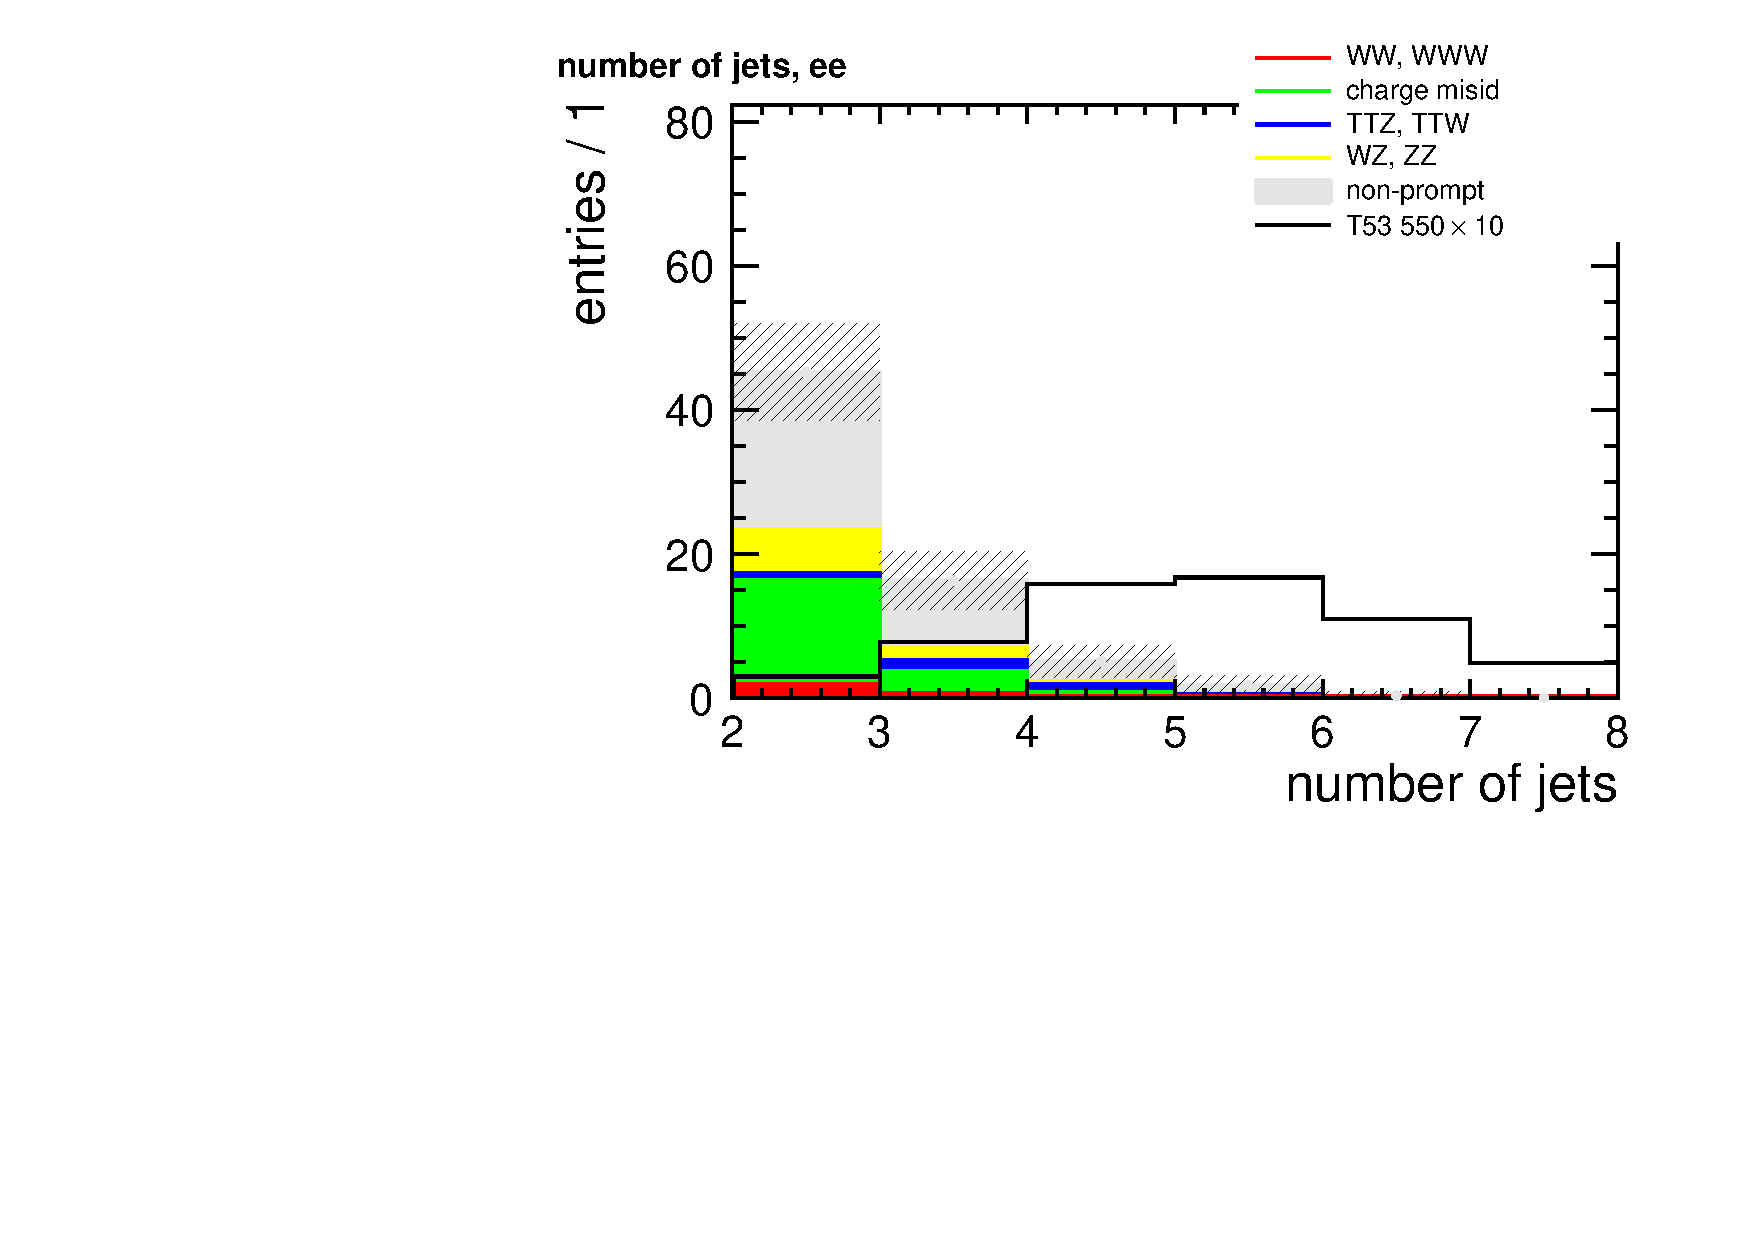
\includegraphics[width=.7\textwidth]{images/pdf/same-sign,_2_jets/n_jets_ee_0}\\
    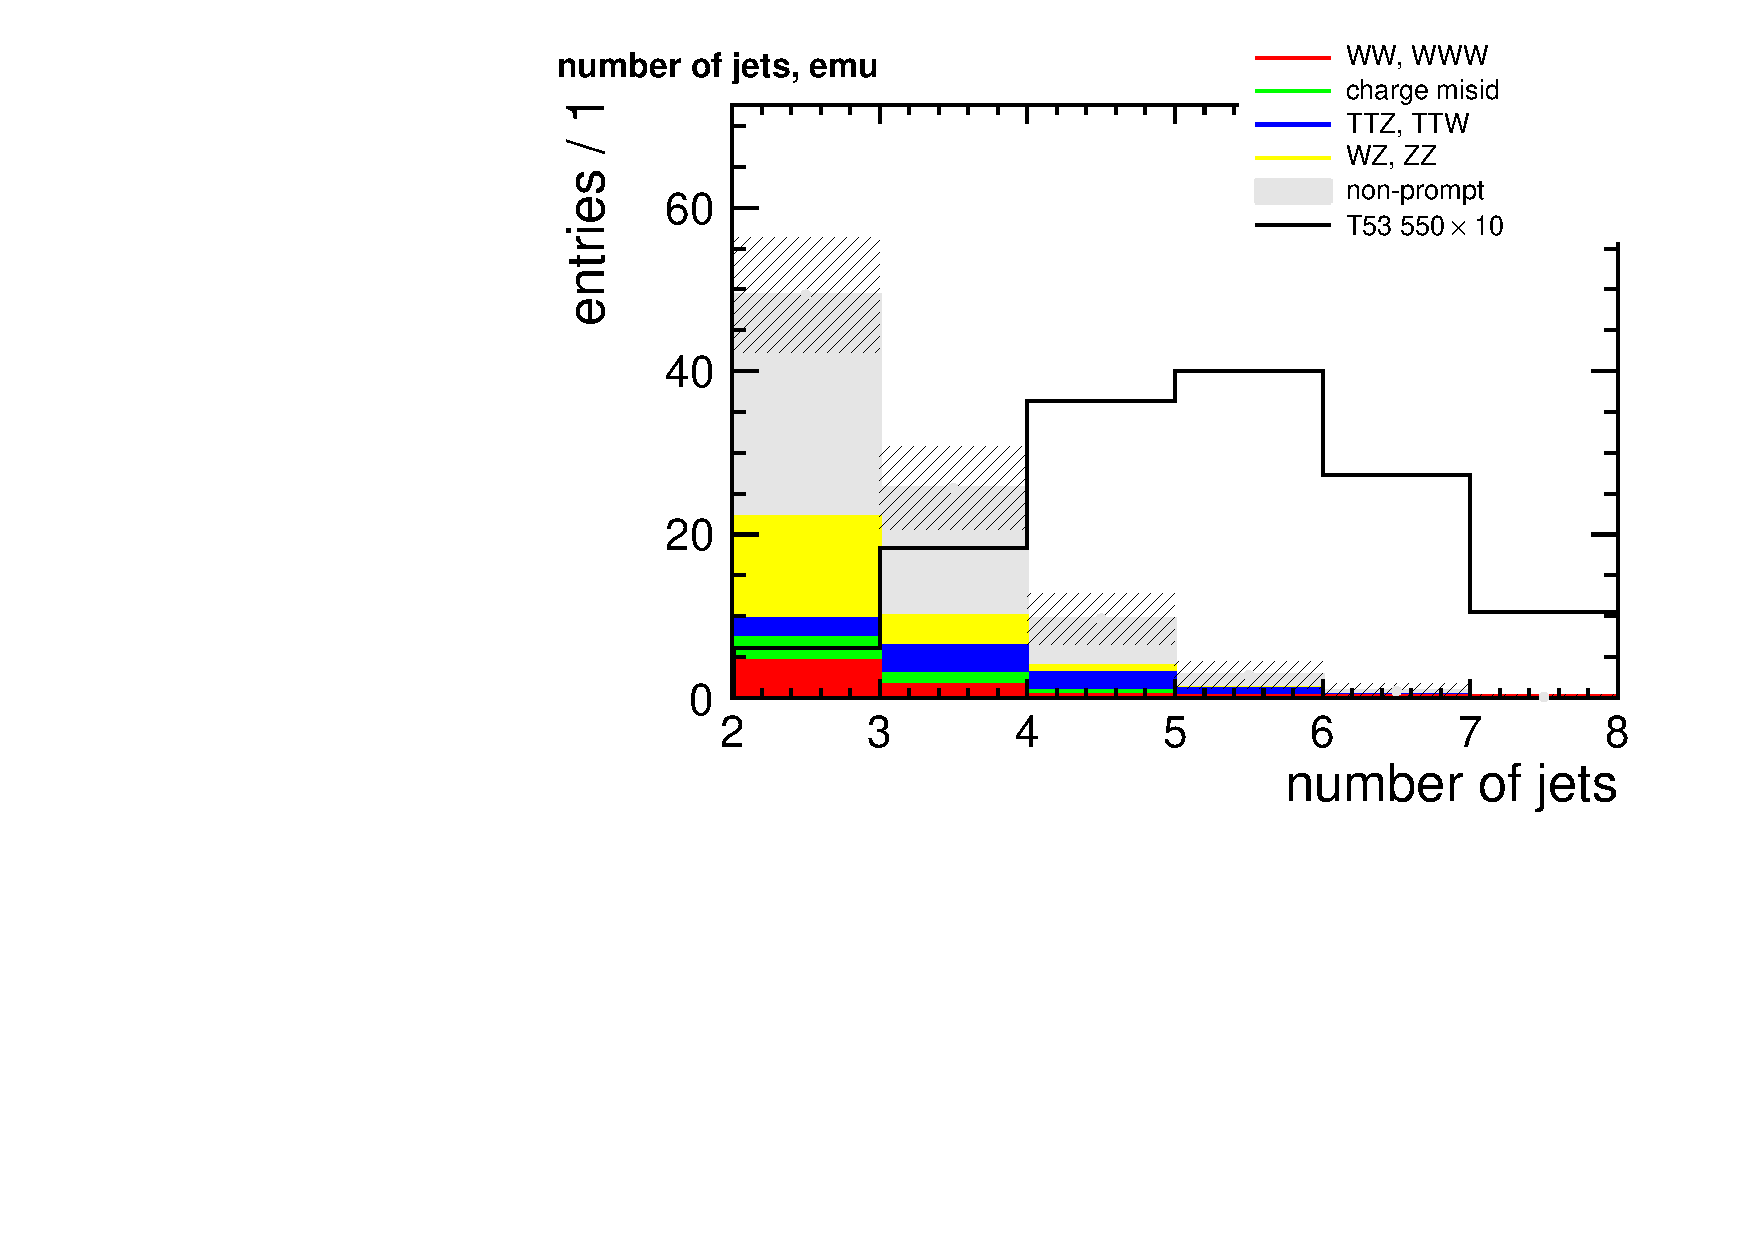
\includegraphics[width=.7\textwidth]{images/pdf/same-sign,_2_jets/n_jets_emu_0}\\
    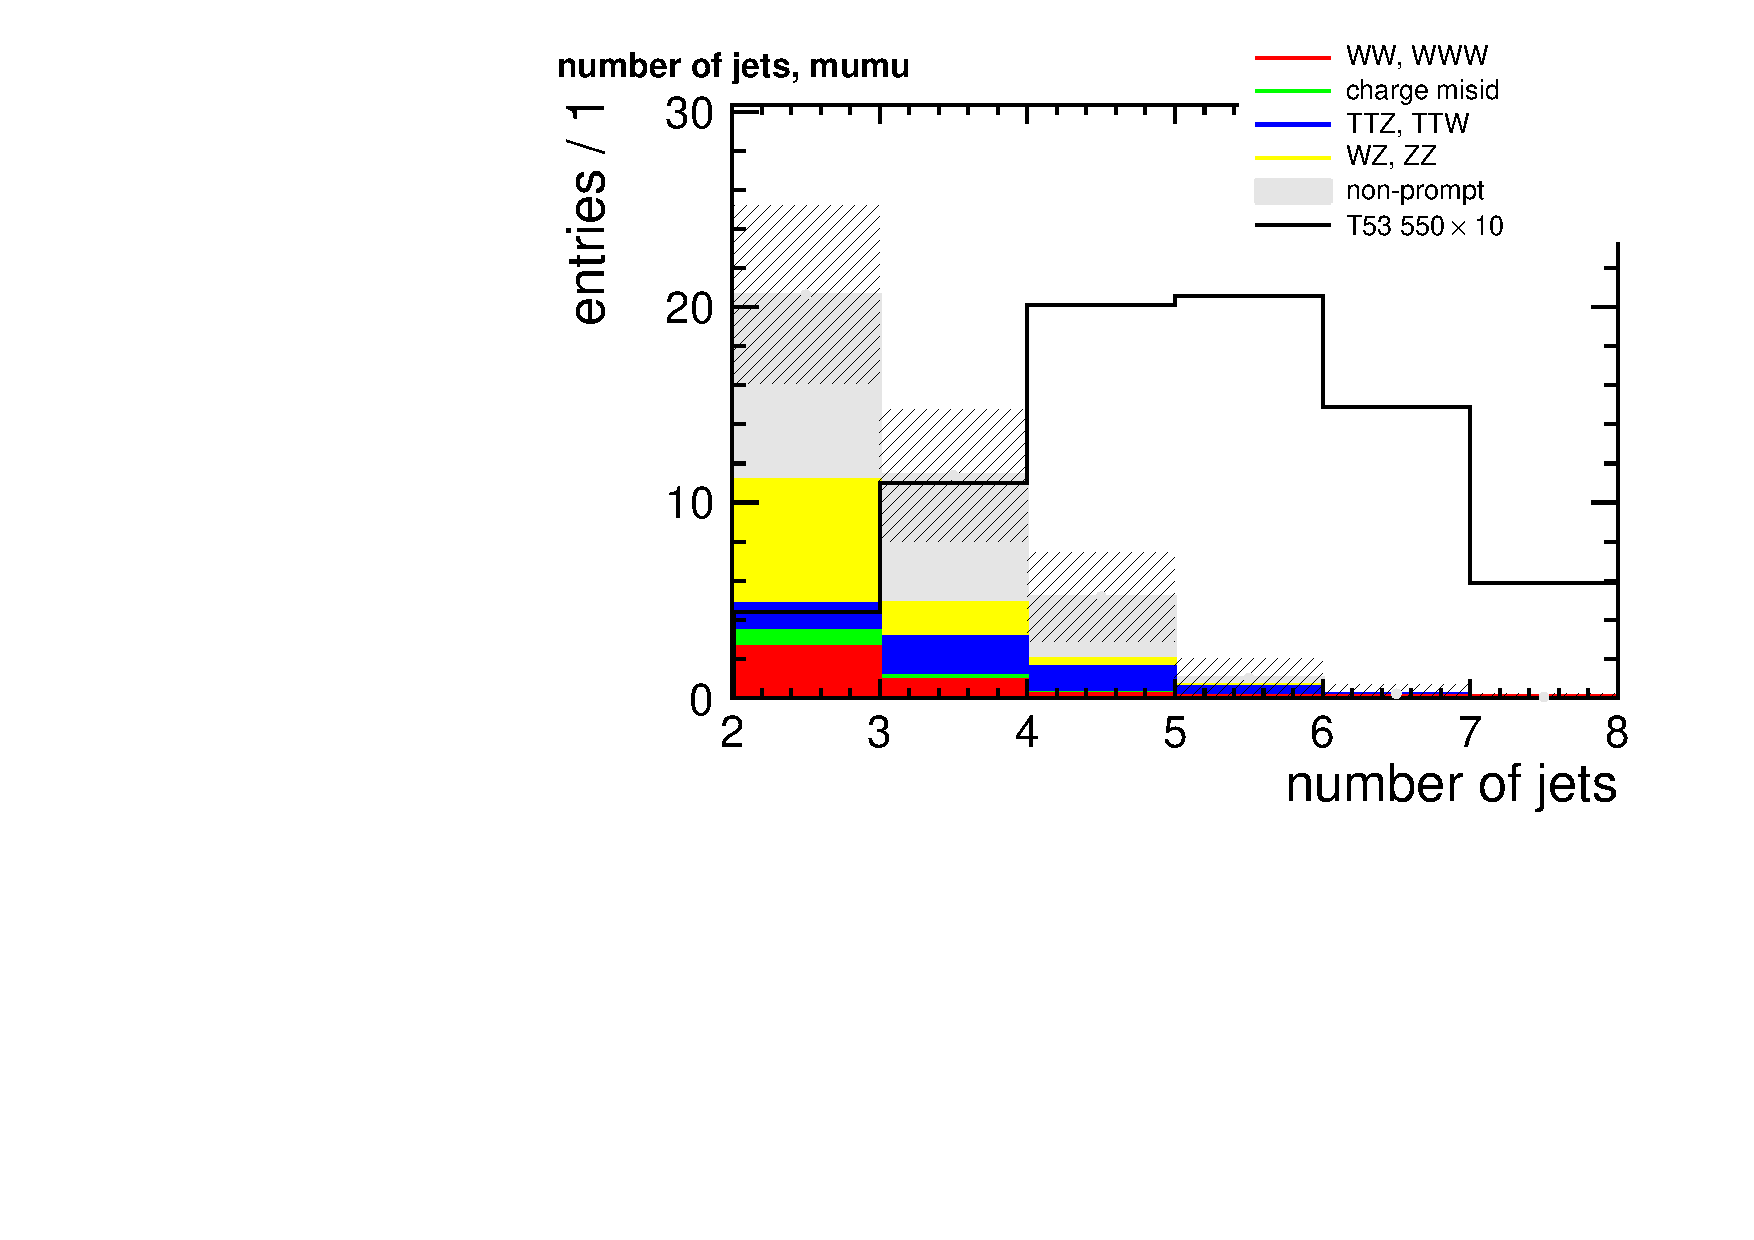
\includegraphics[width=.7\textwidth]{images/pdf/same-sign,_2_jets/n_jets_mumu_0}
    \caption{Events with two same-sign leptons and two jets. Distribution of the number of jets in the backgrounds and
        signal for the \unit[550]{GeV} mass point for the three
        decay channels \E\E, \E\M\ and \M\M. The signal is
    amplified by factor of ten, the data-driven backgrounds for the
non-prompt and charge misidentification contributions are detailed in
chapter~\ref{chap:data_driven}. The shaded area includes statistical and
systematic uncertainties.}
    \label{fig:n_jets_app}
\end{figure}

\begin{figure}[htb]
    \centering
    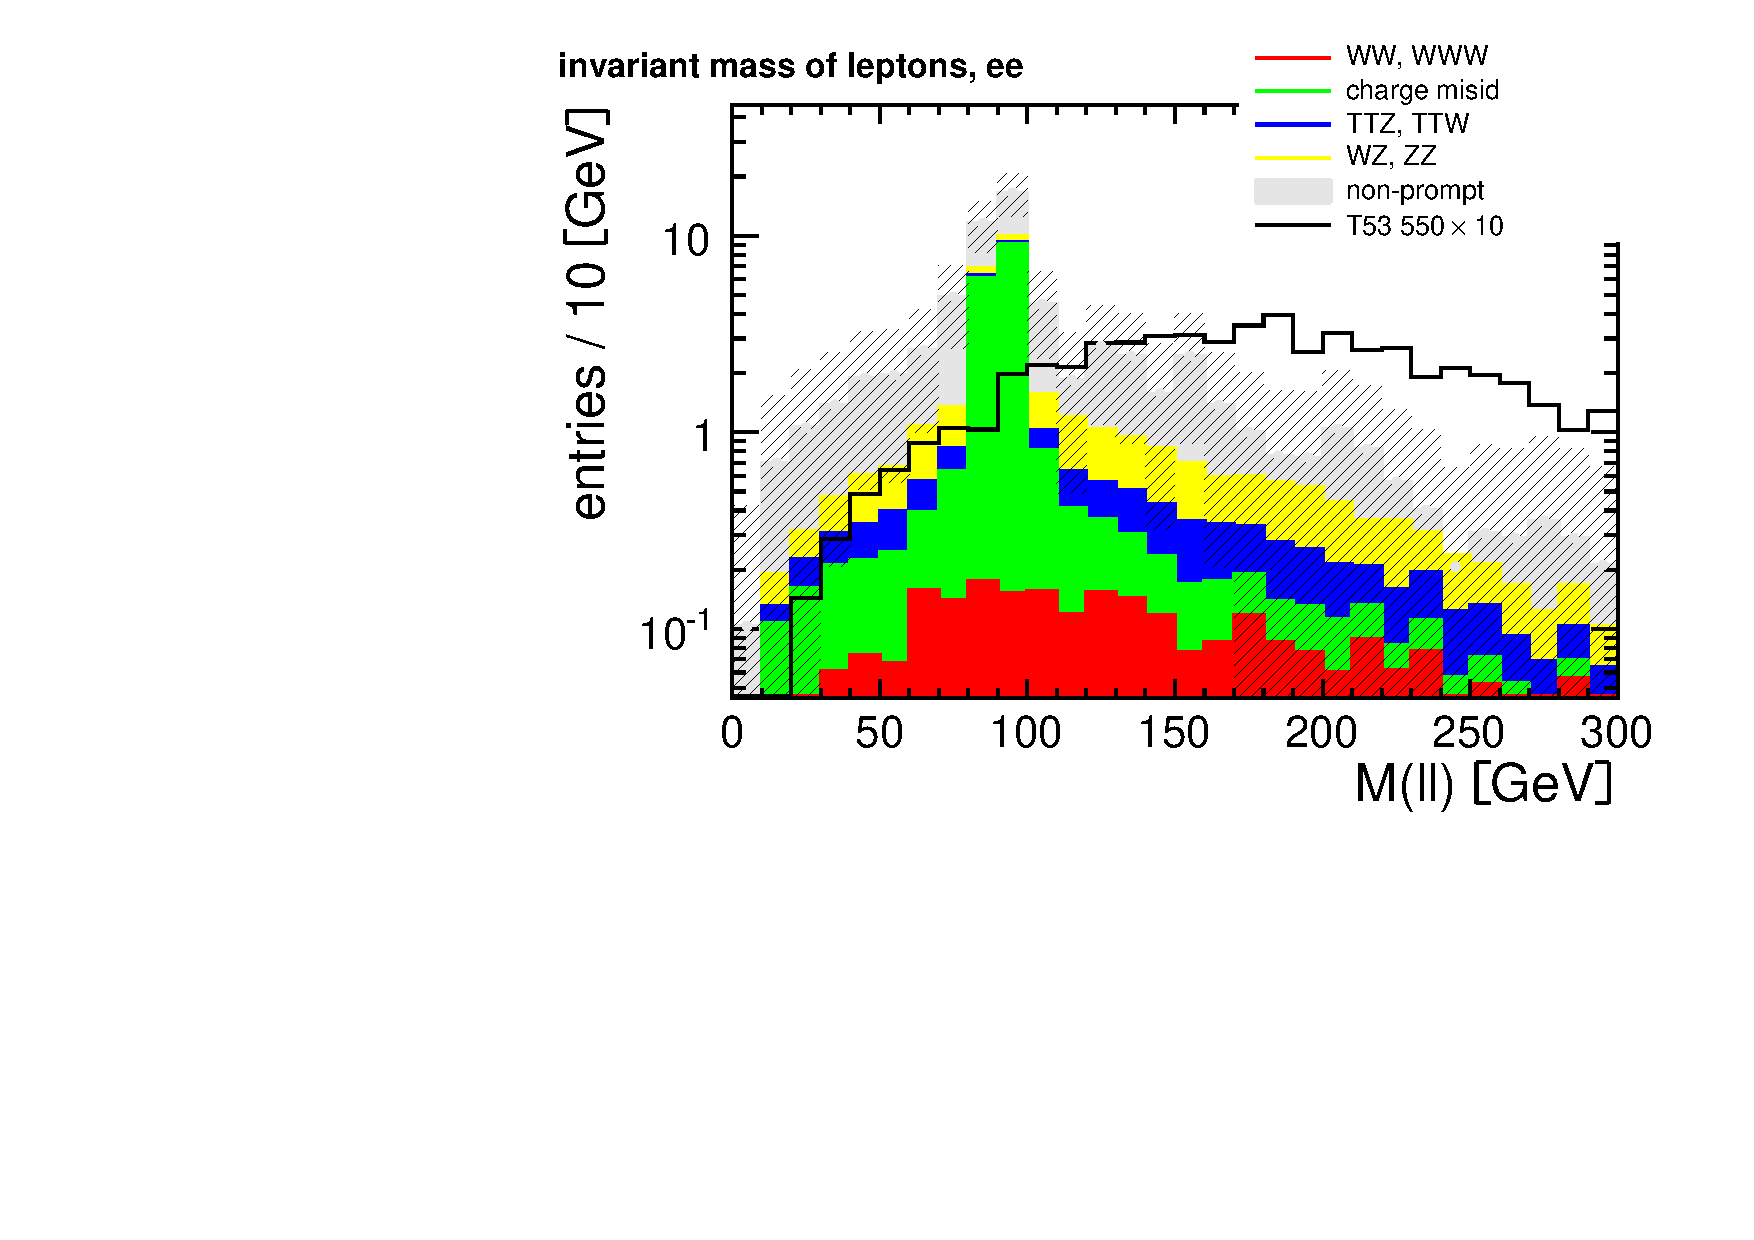
\includegraphics[width=.7\textwidth]{images/pdf/same-sign,_2_jets/lep_mass_ee_0}
    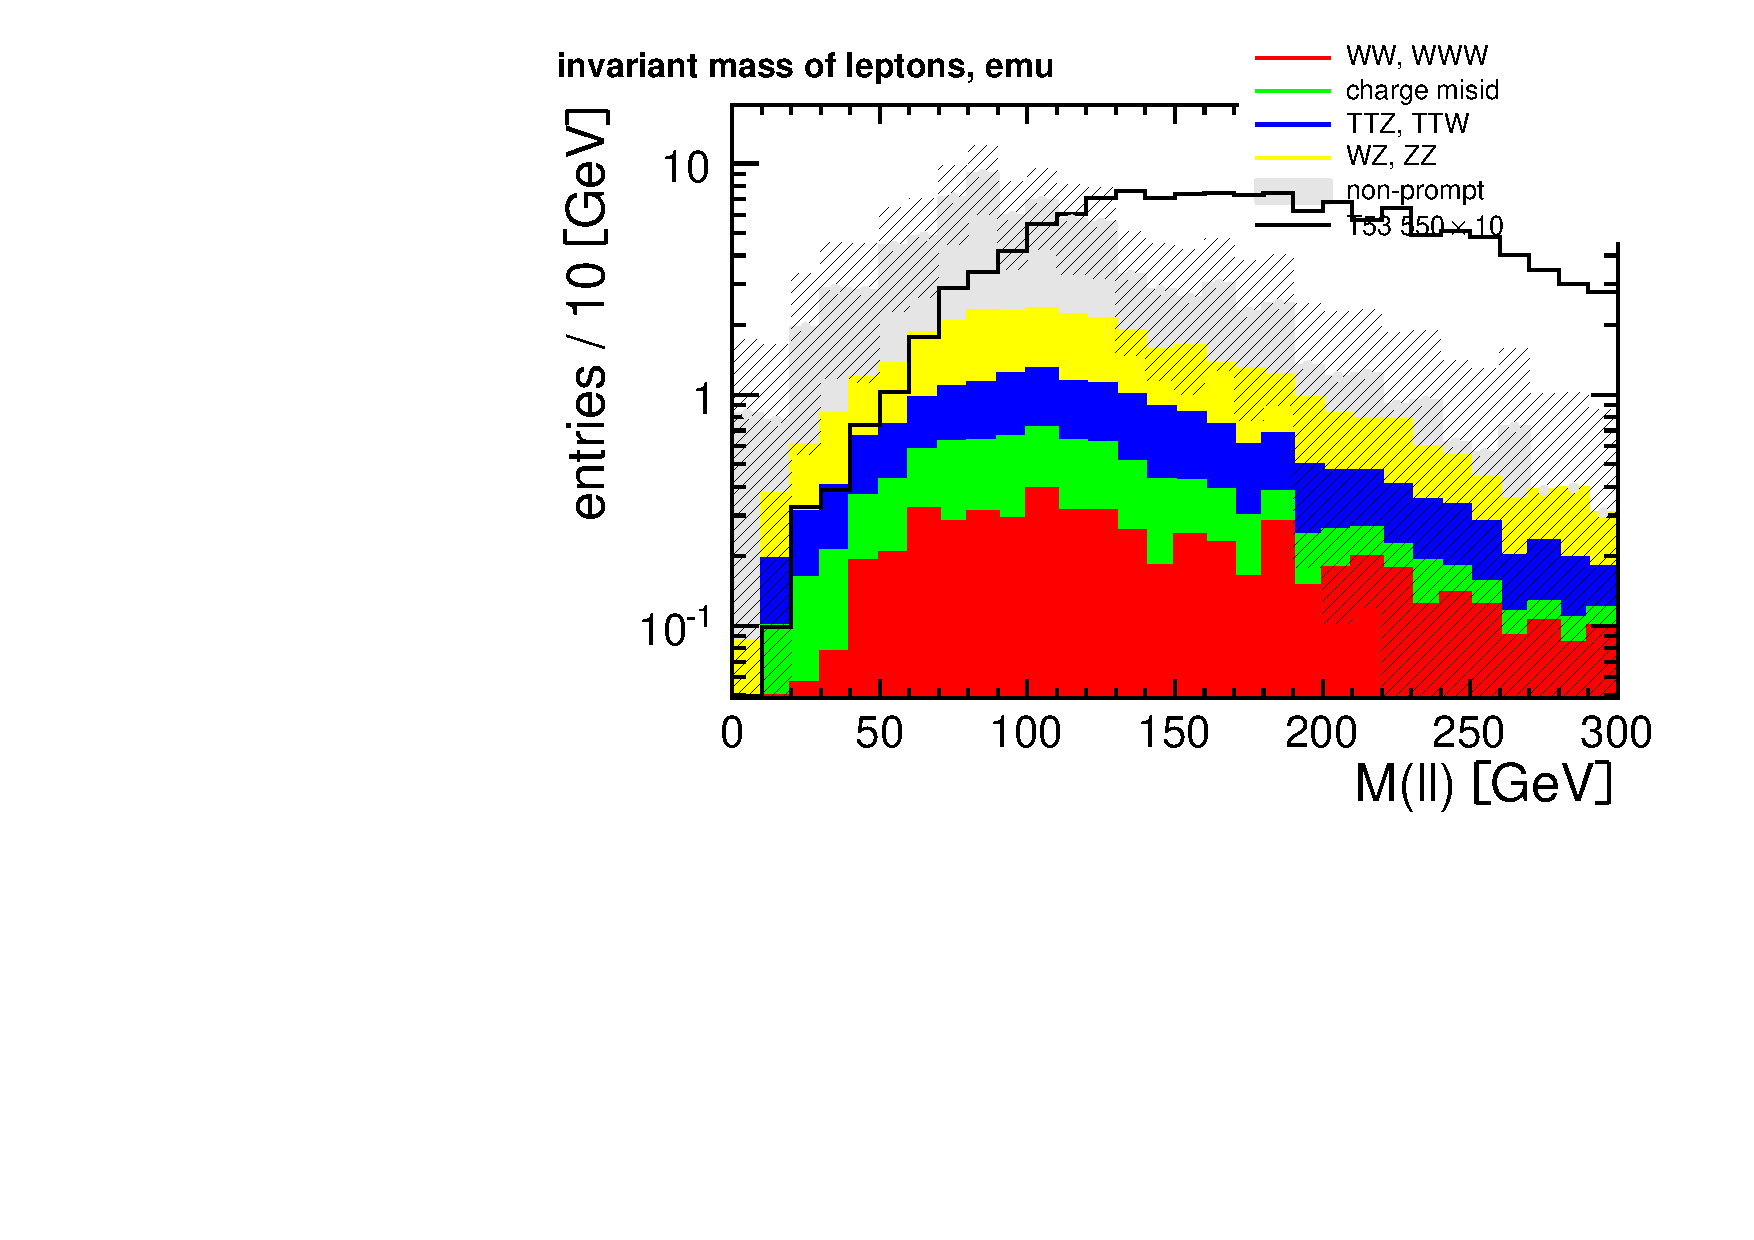
\includegraphics[width=.7\textwidth]{images/pdf/same-sign,_2_jets/lep_mass_emu_0}
    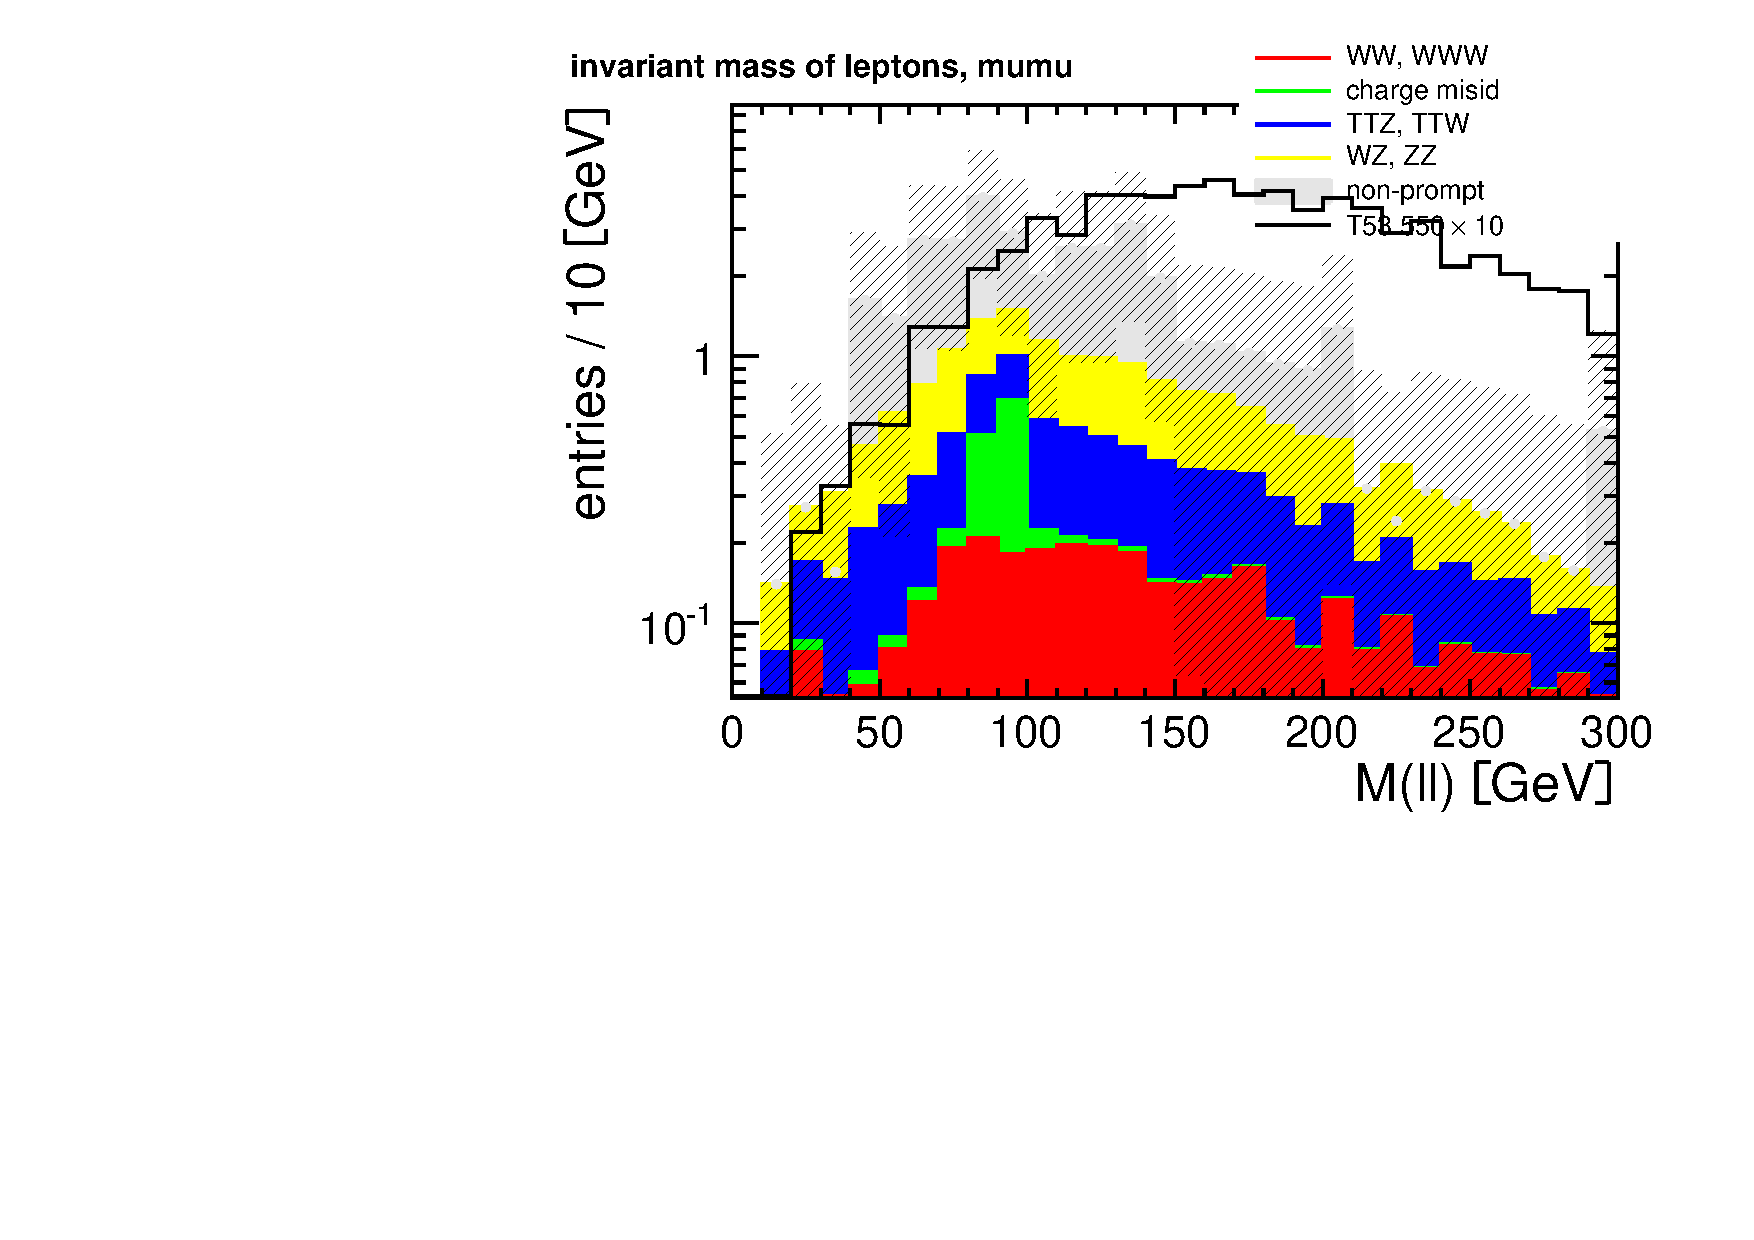
\includegraphics[width=.7\textwidth]{images/pdf/same-sign,_2_jets/lep_mass_mumu_0}
    \caption{Events with two same-sign leptons and two jets. Distribution of the invariant mass of the leptons in the backgrounds and
        signal for the \unit[550]{GeV} mass point for the three
        decay channels \E\E, \E\M\ and \M\M. The signal is
    amplified by factor of ten, the data-driven backgrounds for the
non-prompt and charge misidentification contributions are detailed in
chapter~\ref{chap:data_driven}. The shaded area includes statistical and
systematic uncertainties.}
    \label{fig:lep_mass_app}
\end{figure}

\begin{figure}[htb]
    \centering
    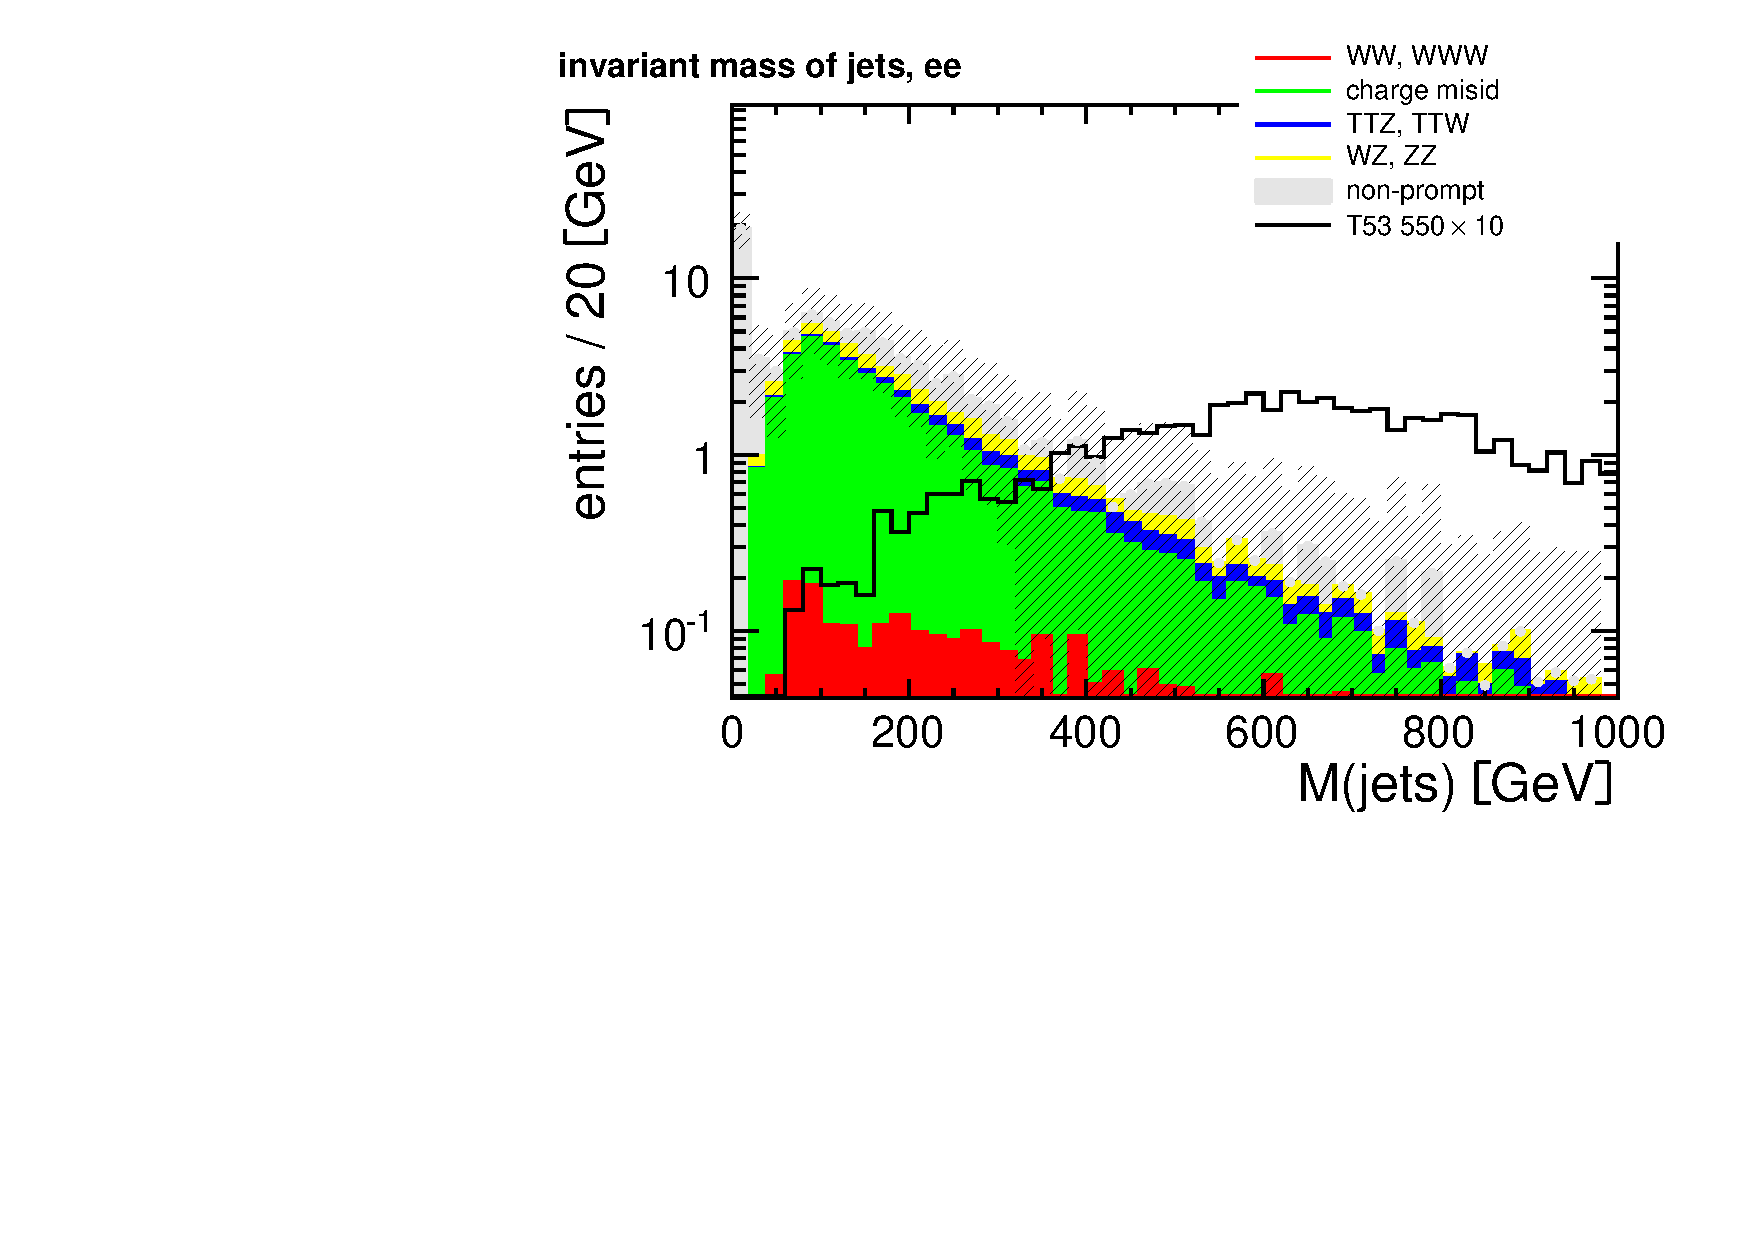
\includegraphics[width=.7\textwidth]{images/pdf/had_mass_ee_0}
    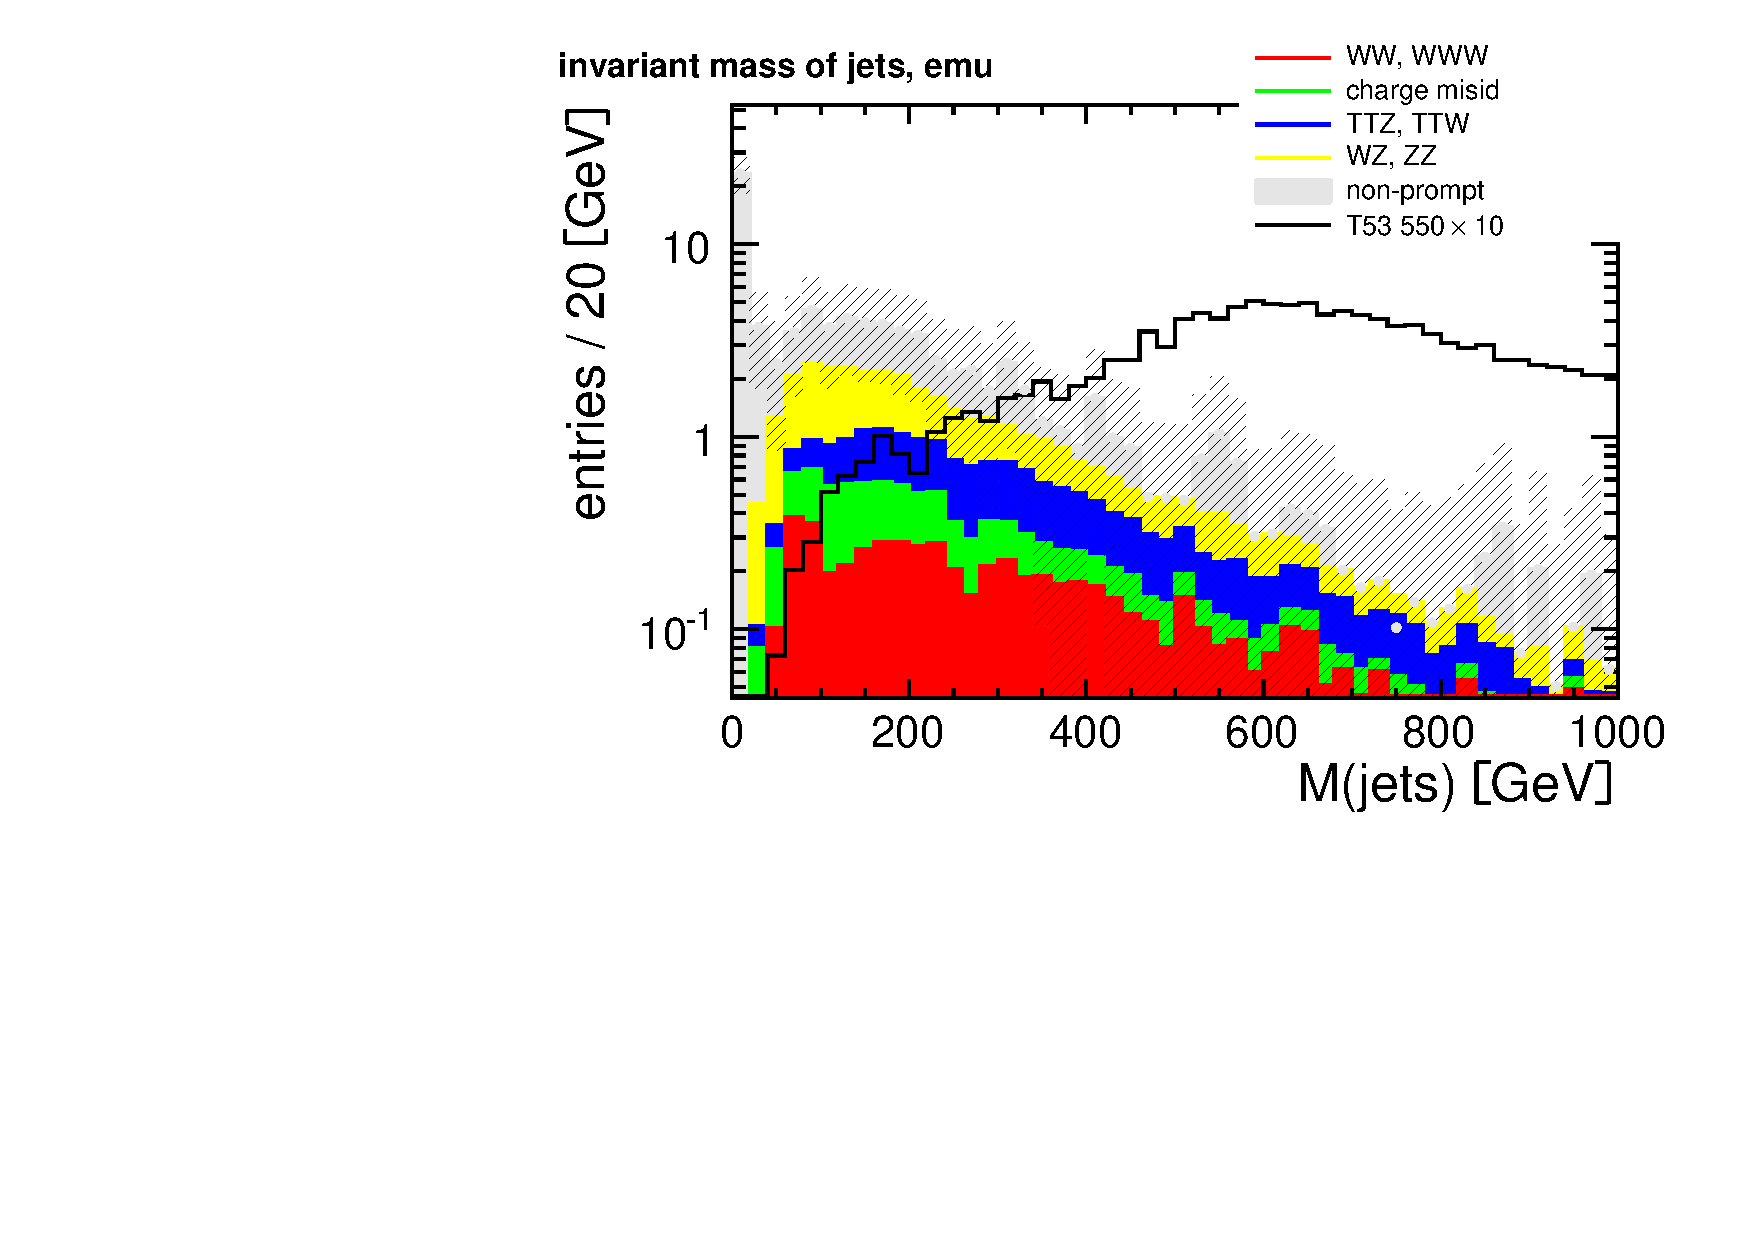
\includegraphics[width=.7\textwidth]{images/pdf/had_mass_emu_0}
    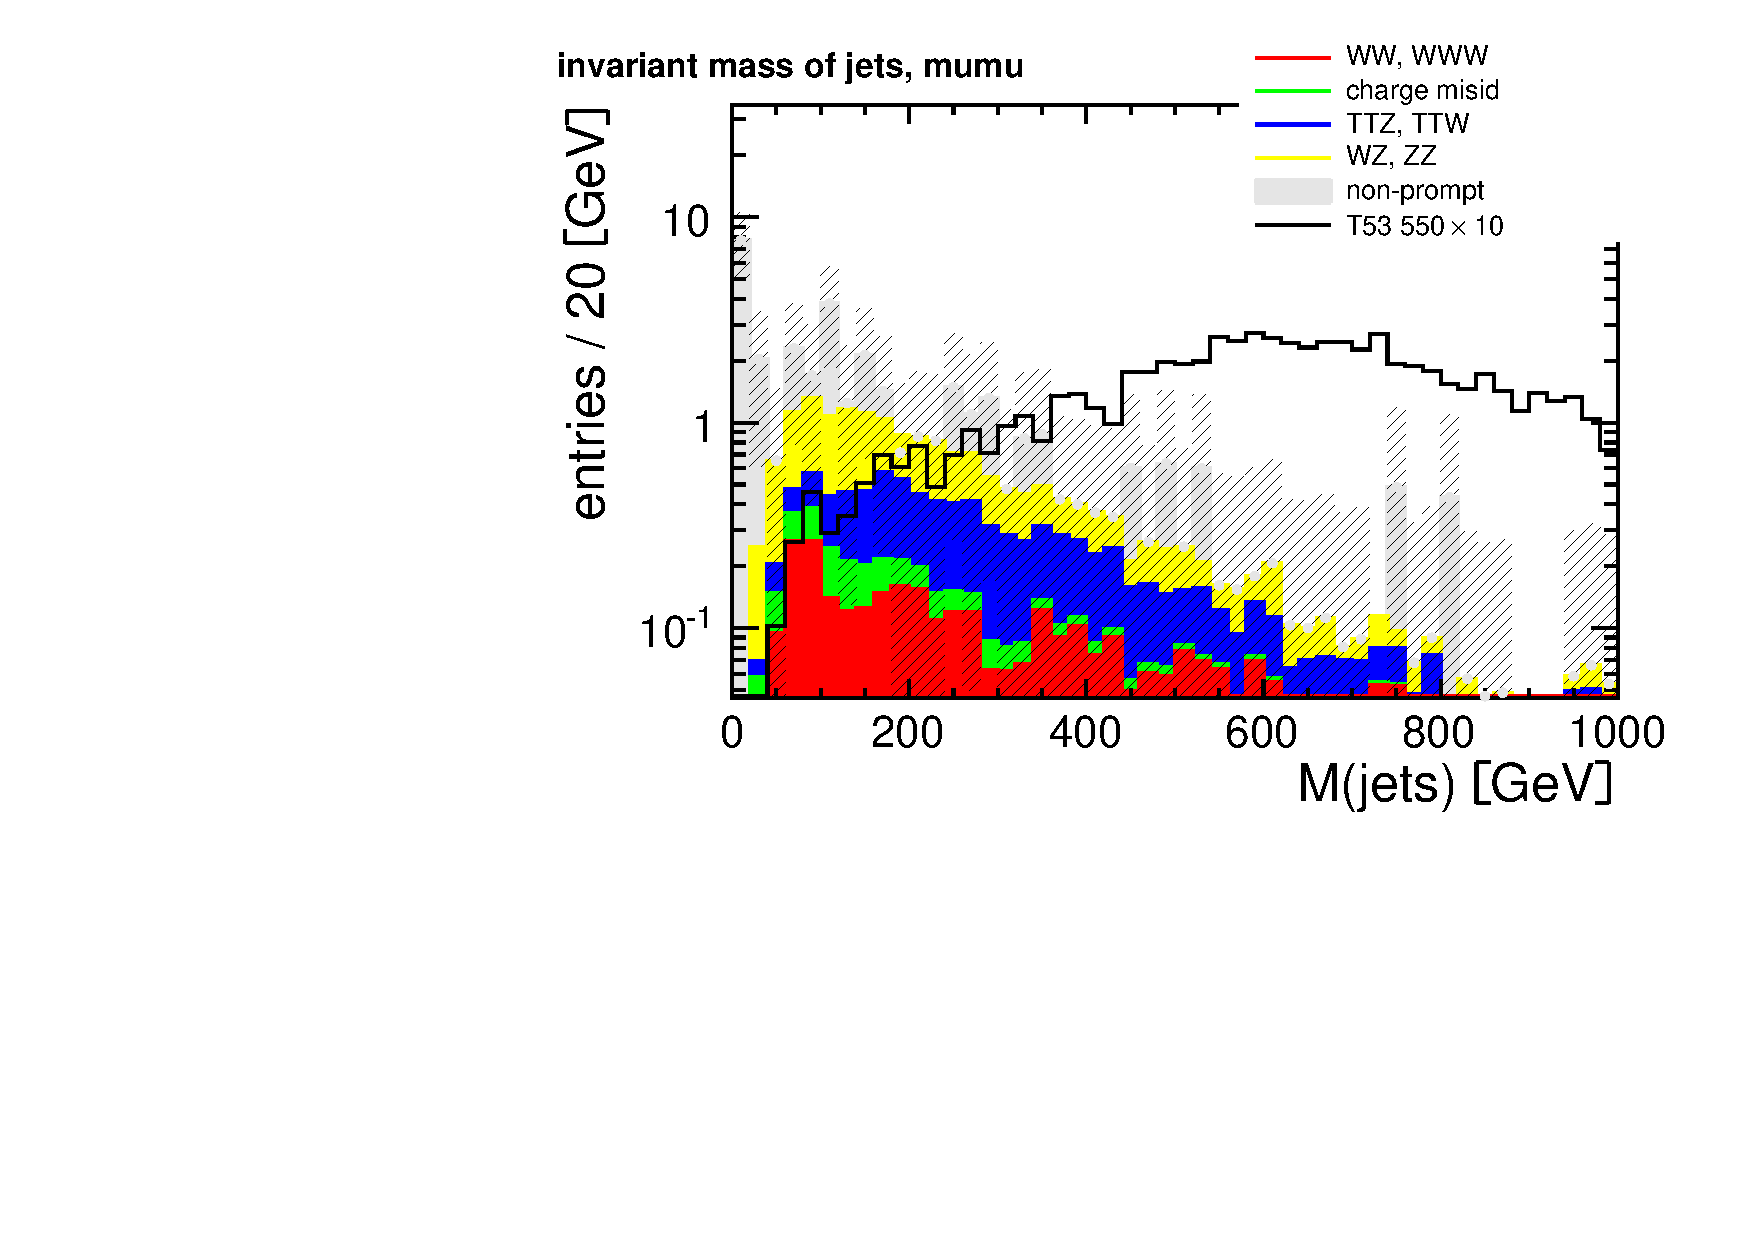
\includegraphics[width=.7\textwidth]{images/pdf/had_mass_mumu_0}
    \caption{Invariant mass of the hadronic system for the three decay
    channels. Events with two same-sign leptons and at least
two jets are shown.}
    \label{fig:had_mass_app}
\end{figure}

\begin{figure}[htb]
    \centering
    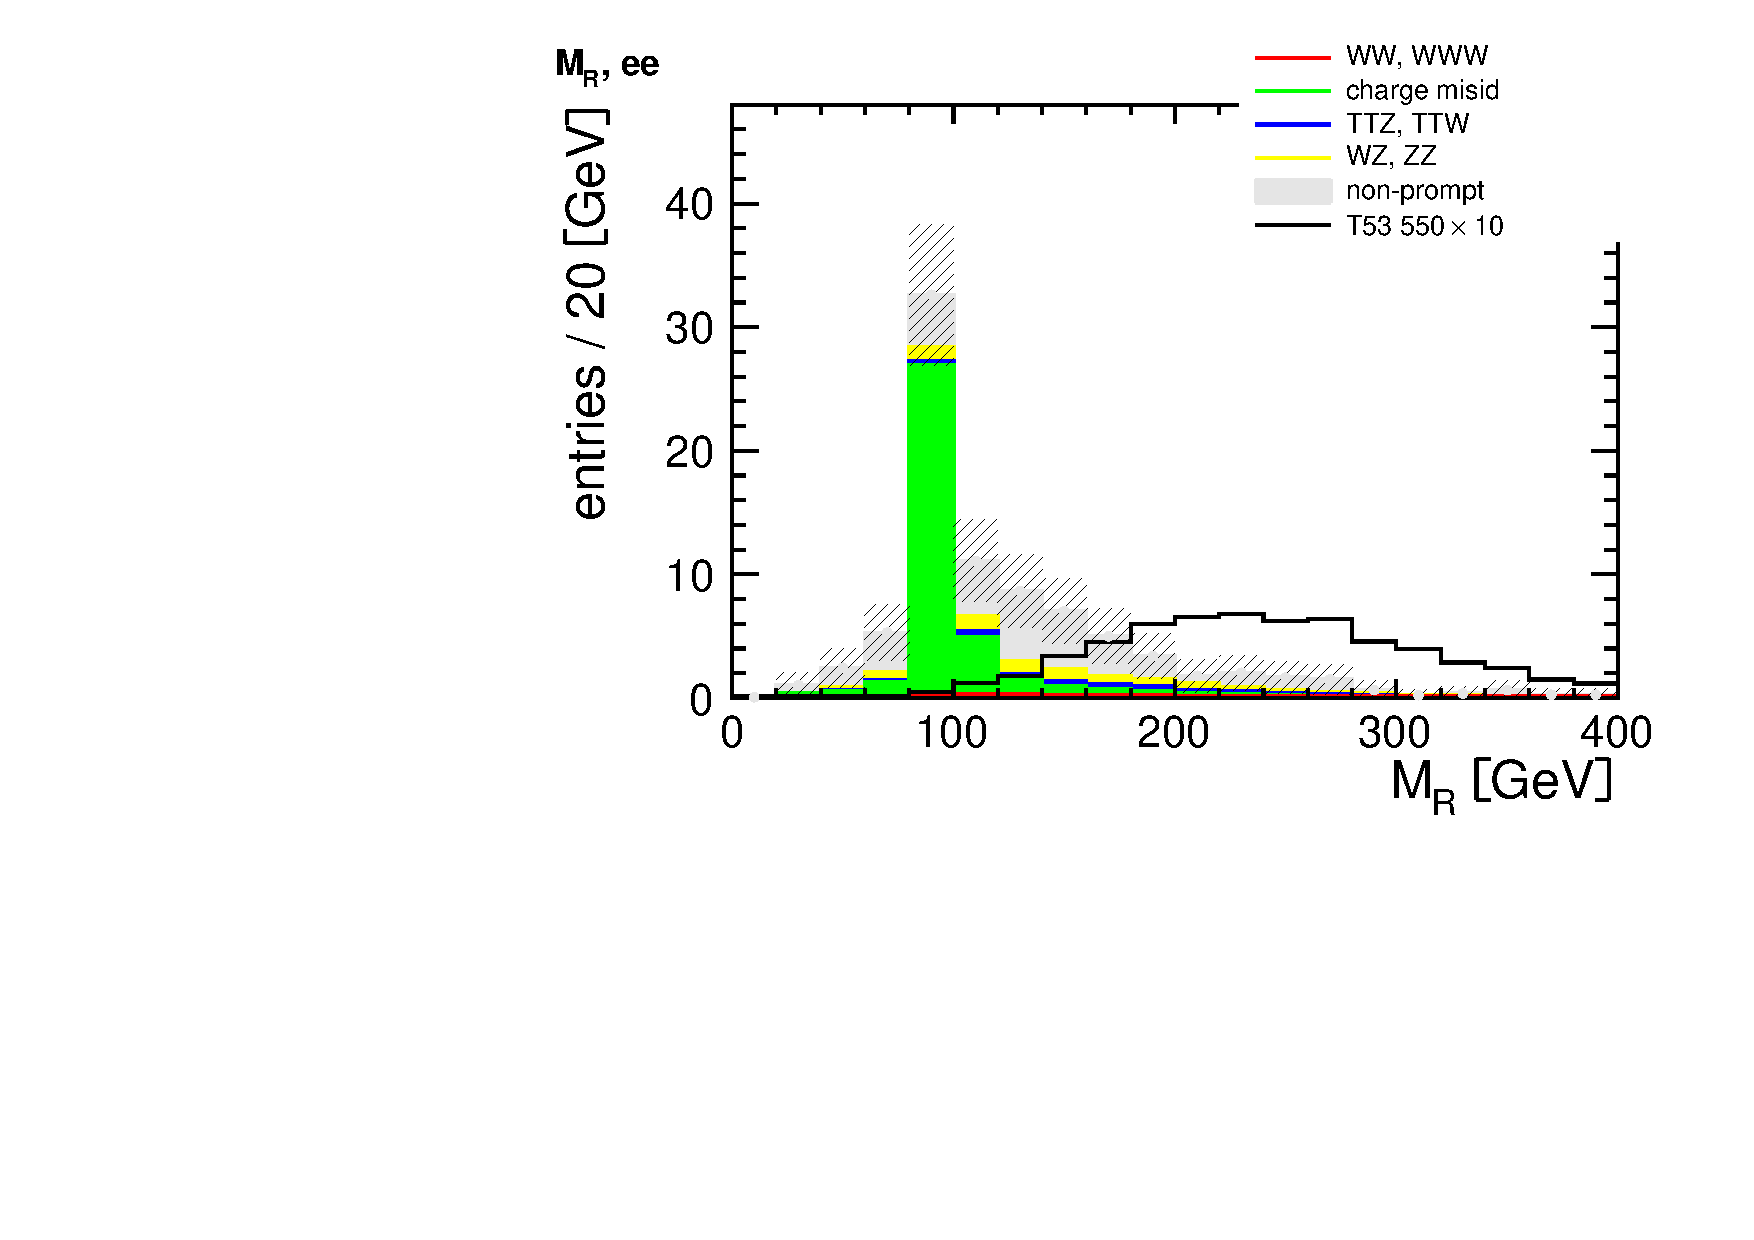
\includegraphics[width=.7\textwidth]{images/pdf/mr_ee_0}
    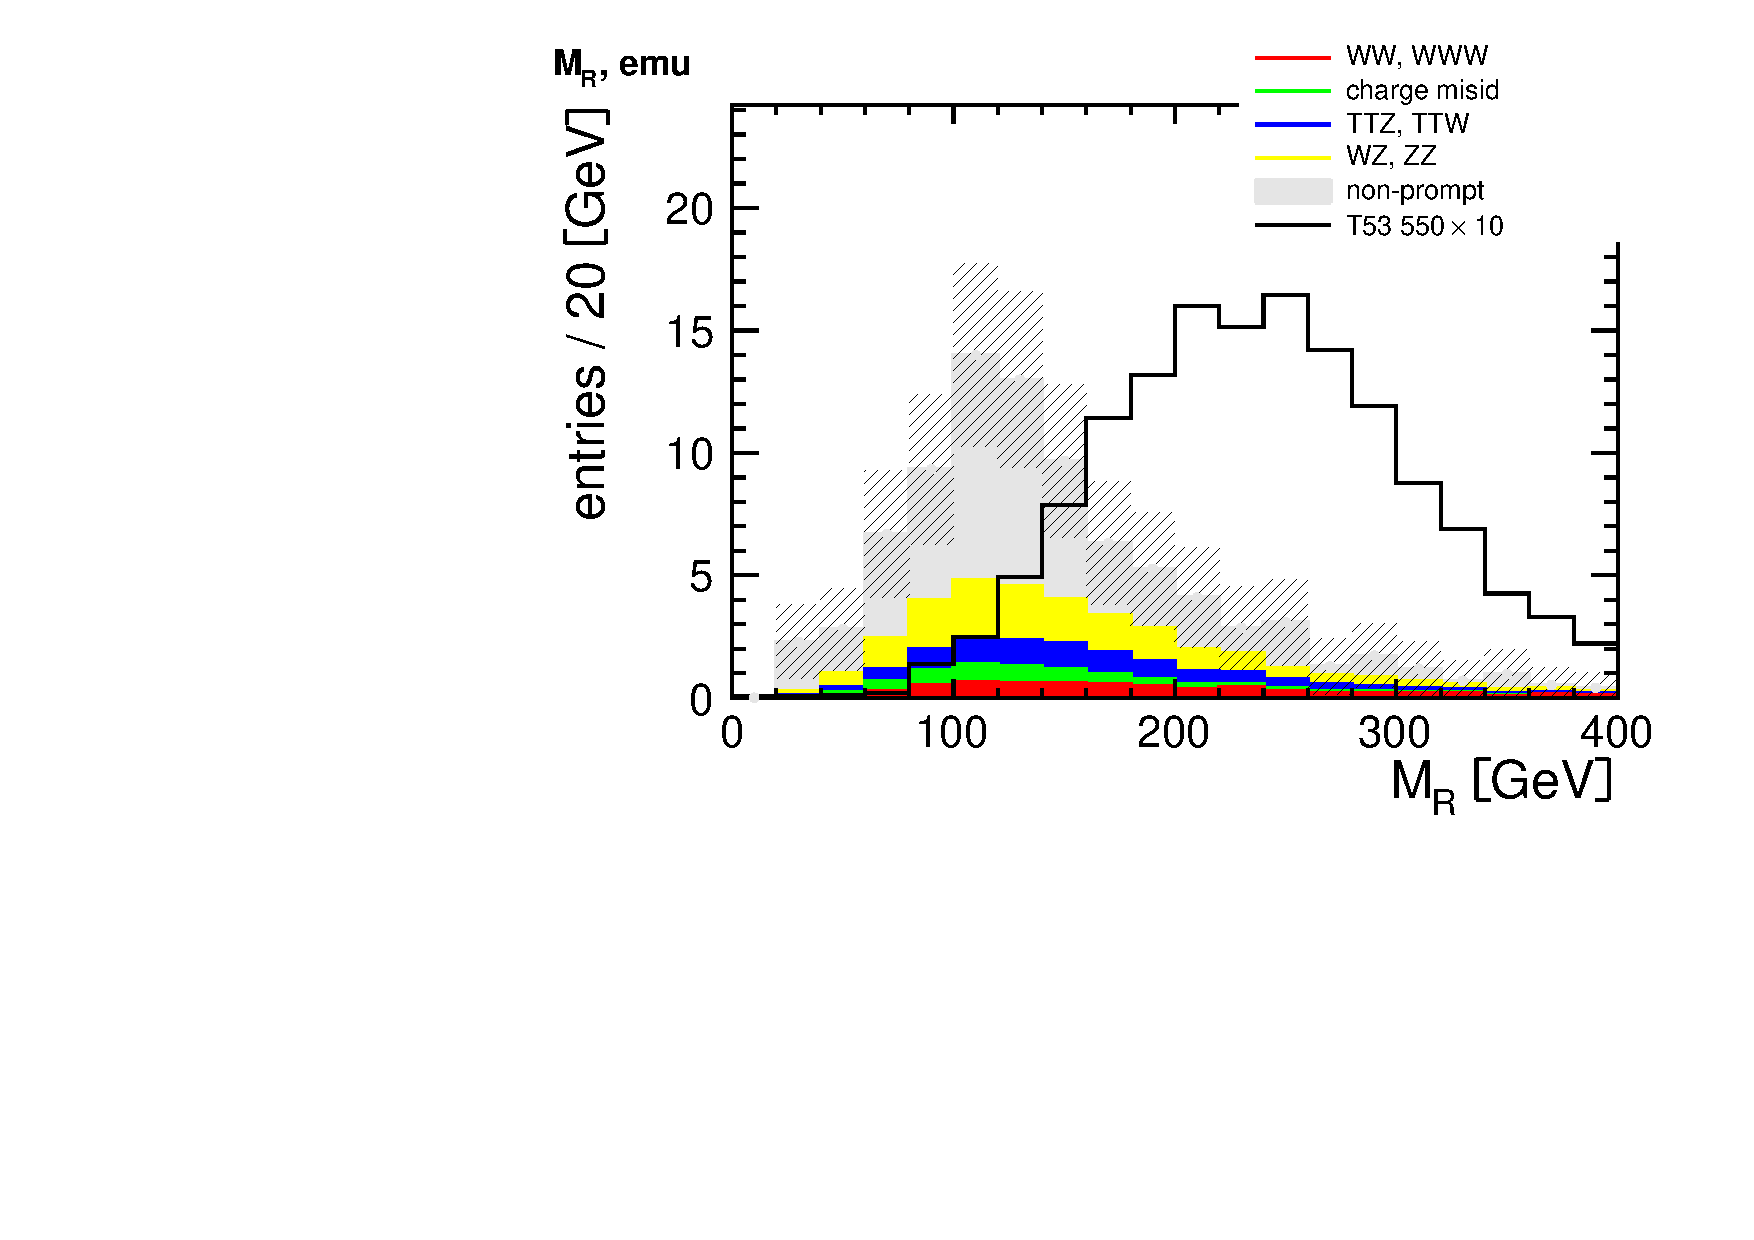
\includegraphics[width=.7\textwidth]{images/pdf/mr_emu_0}
    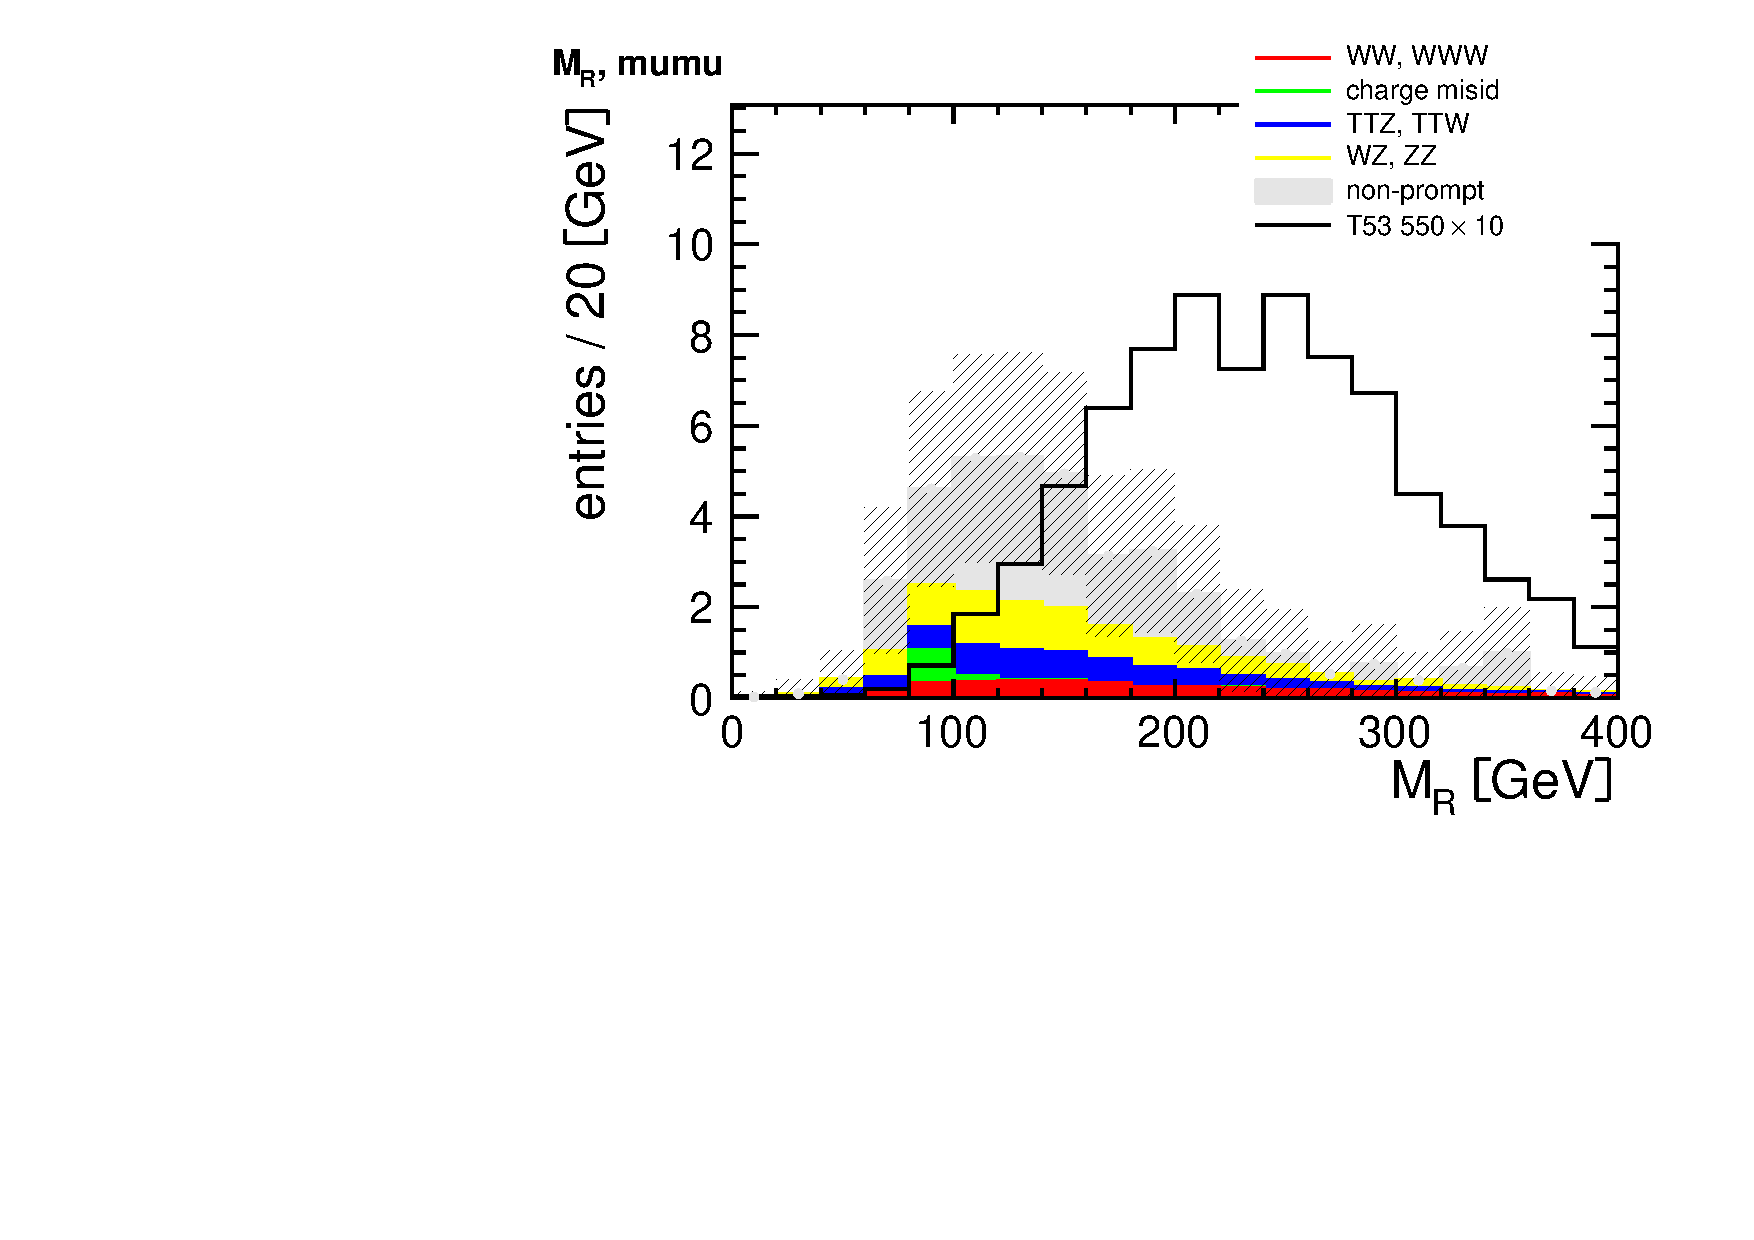
\includegraphics[width=.7\textwidth]{images/pdf/mr_mumu_0}
    \caption{$M_R$ distributions for the three decay channels. Events with two same-sign leptons and at least
two jets are shown.}
    \label{fig:mr_nobtag_app}
\end{figure}

\begin{figure}[htb]
    \centering
    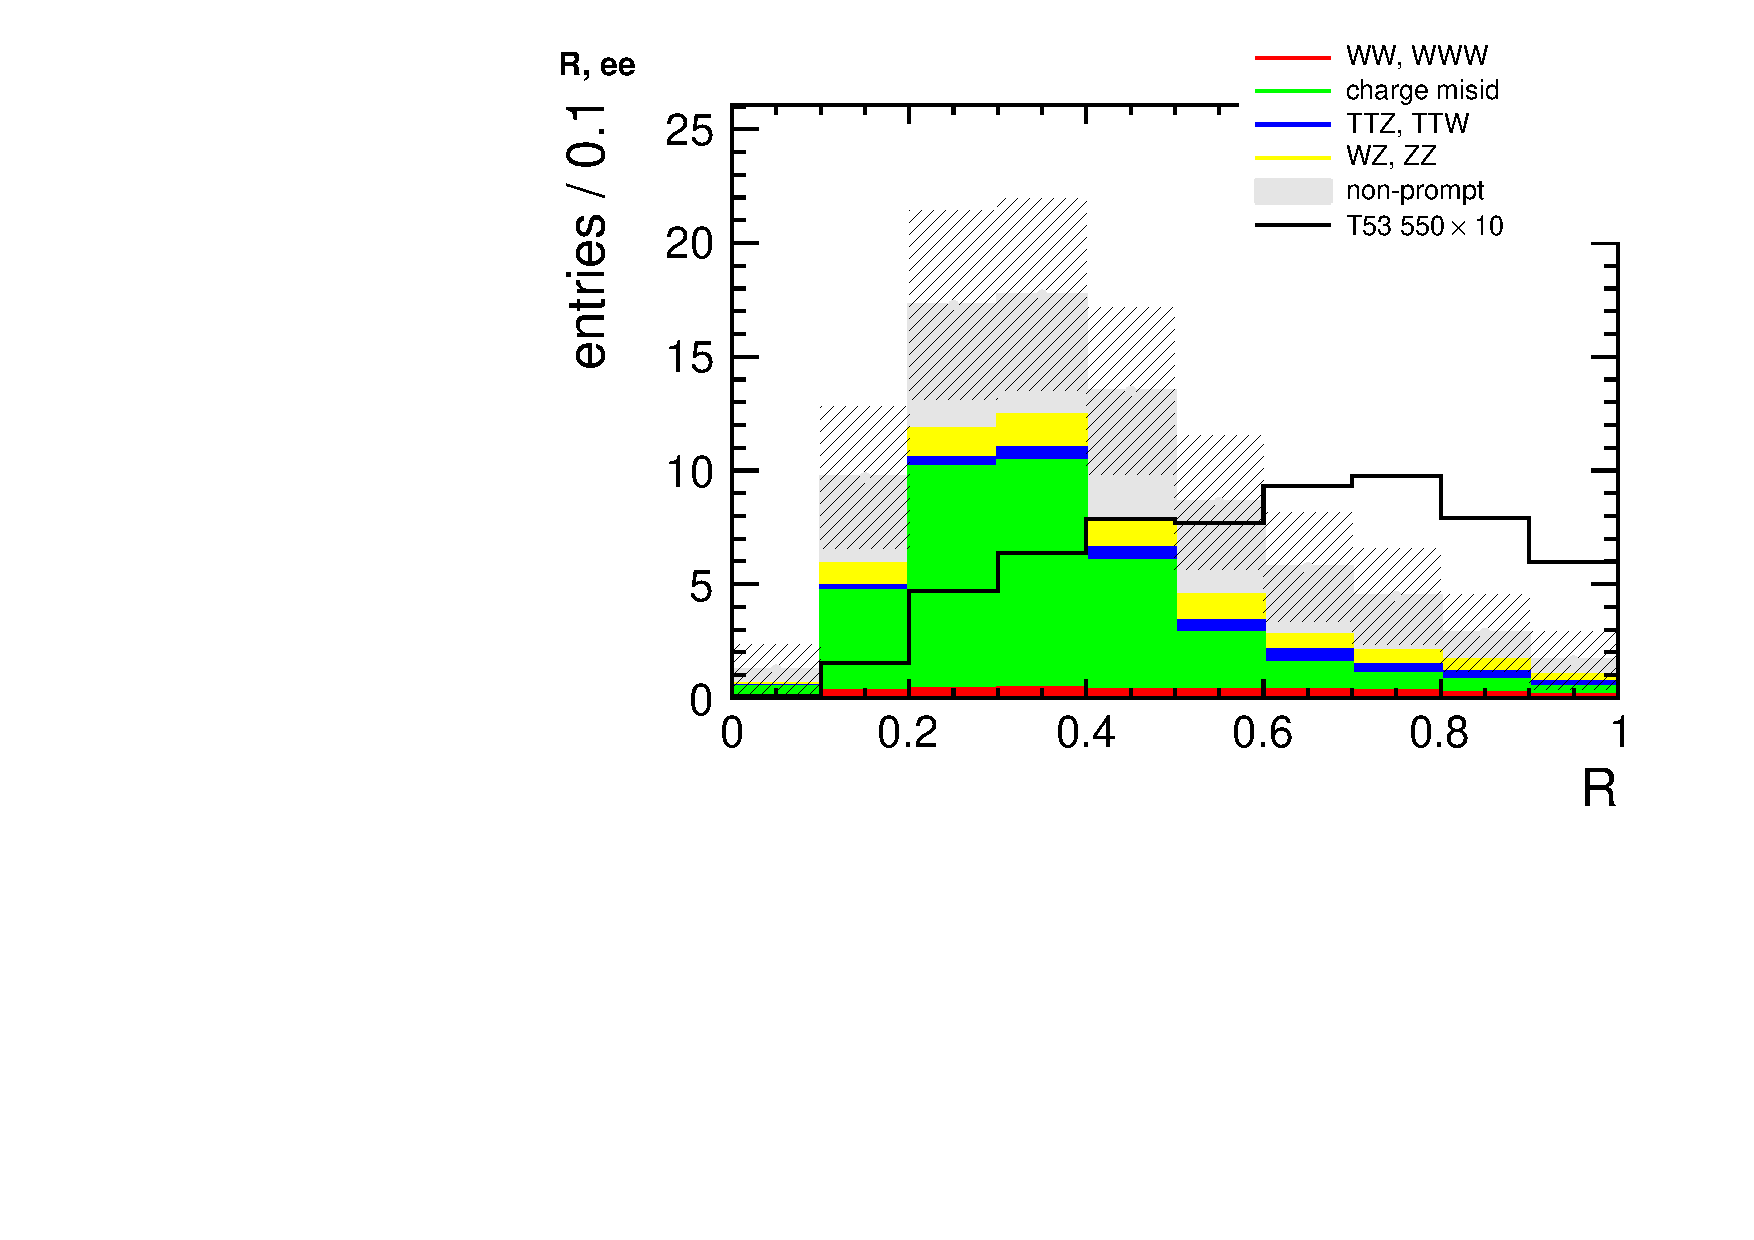
\includegraphics[width=.7\textwidth]{images/pdf/r_ee_0}
    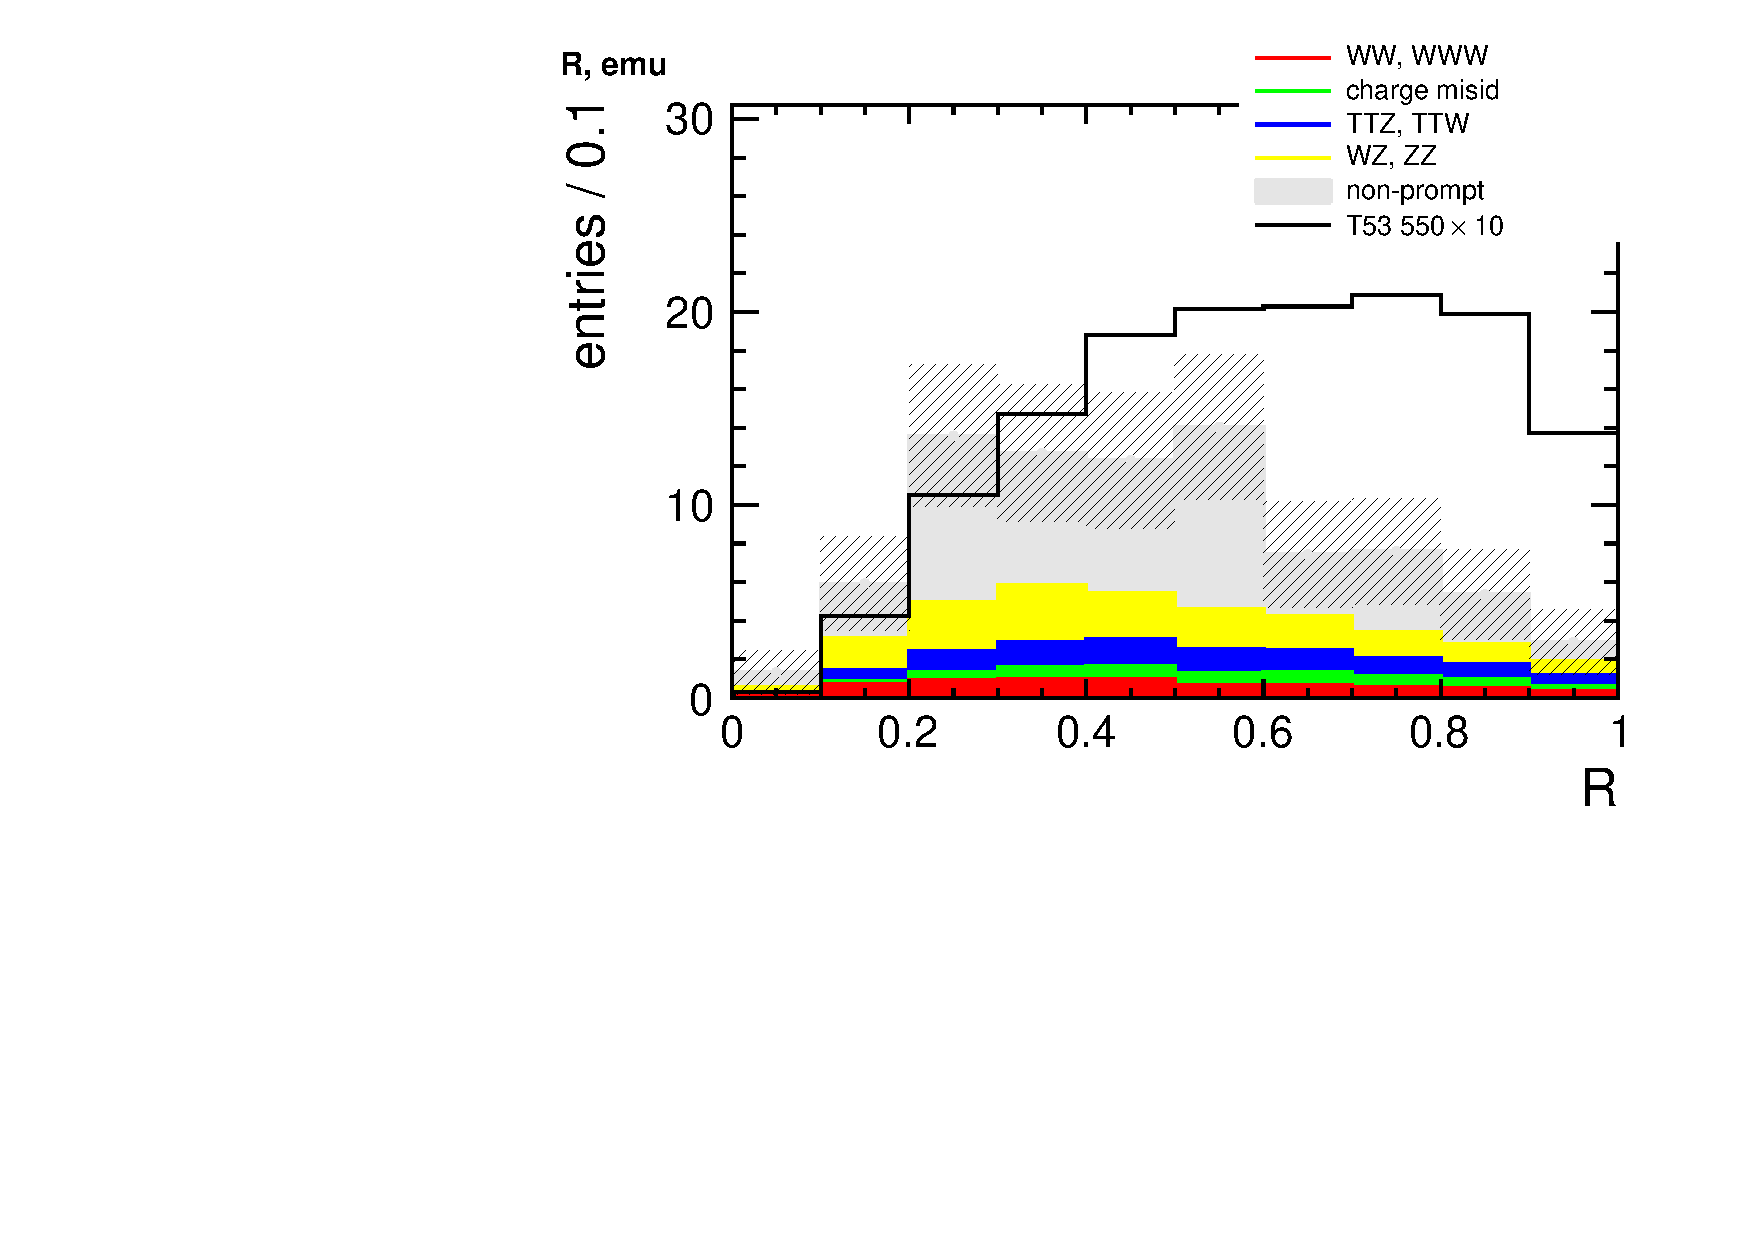
\includegraphics[width=.7\textwidth]{images/pdf/r_emu_0}
    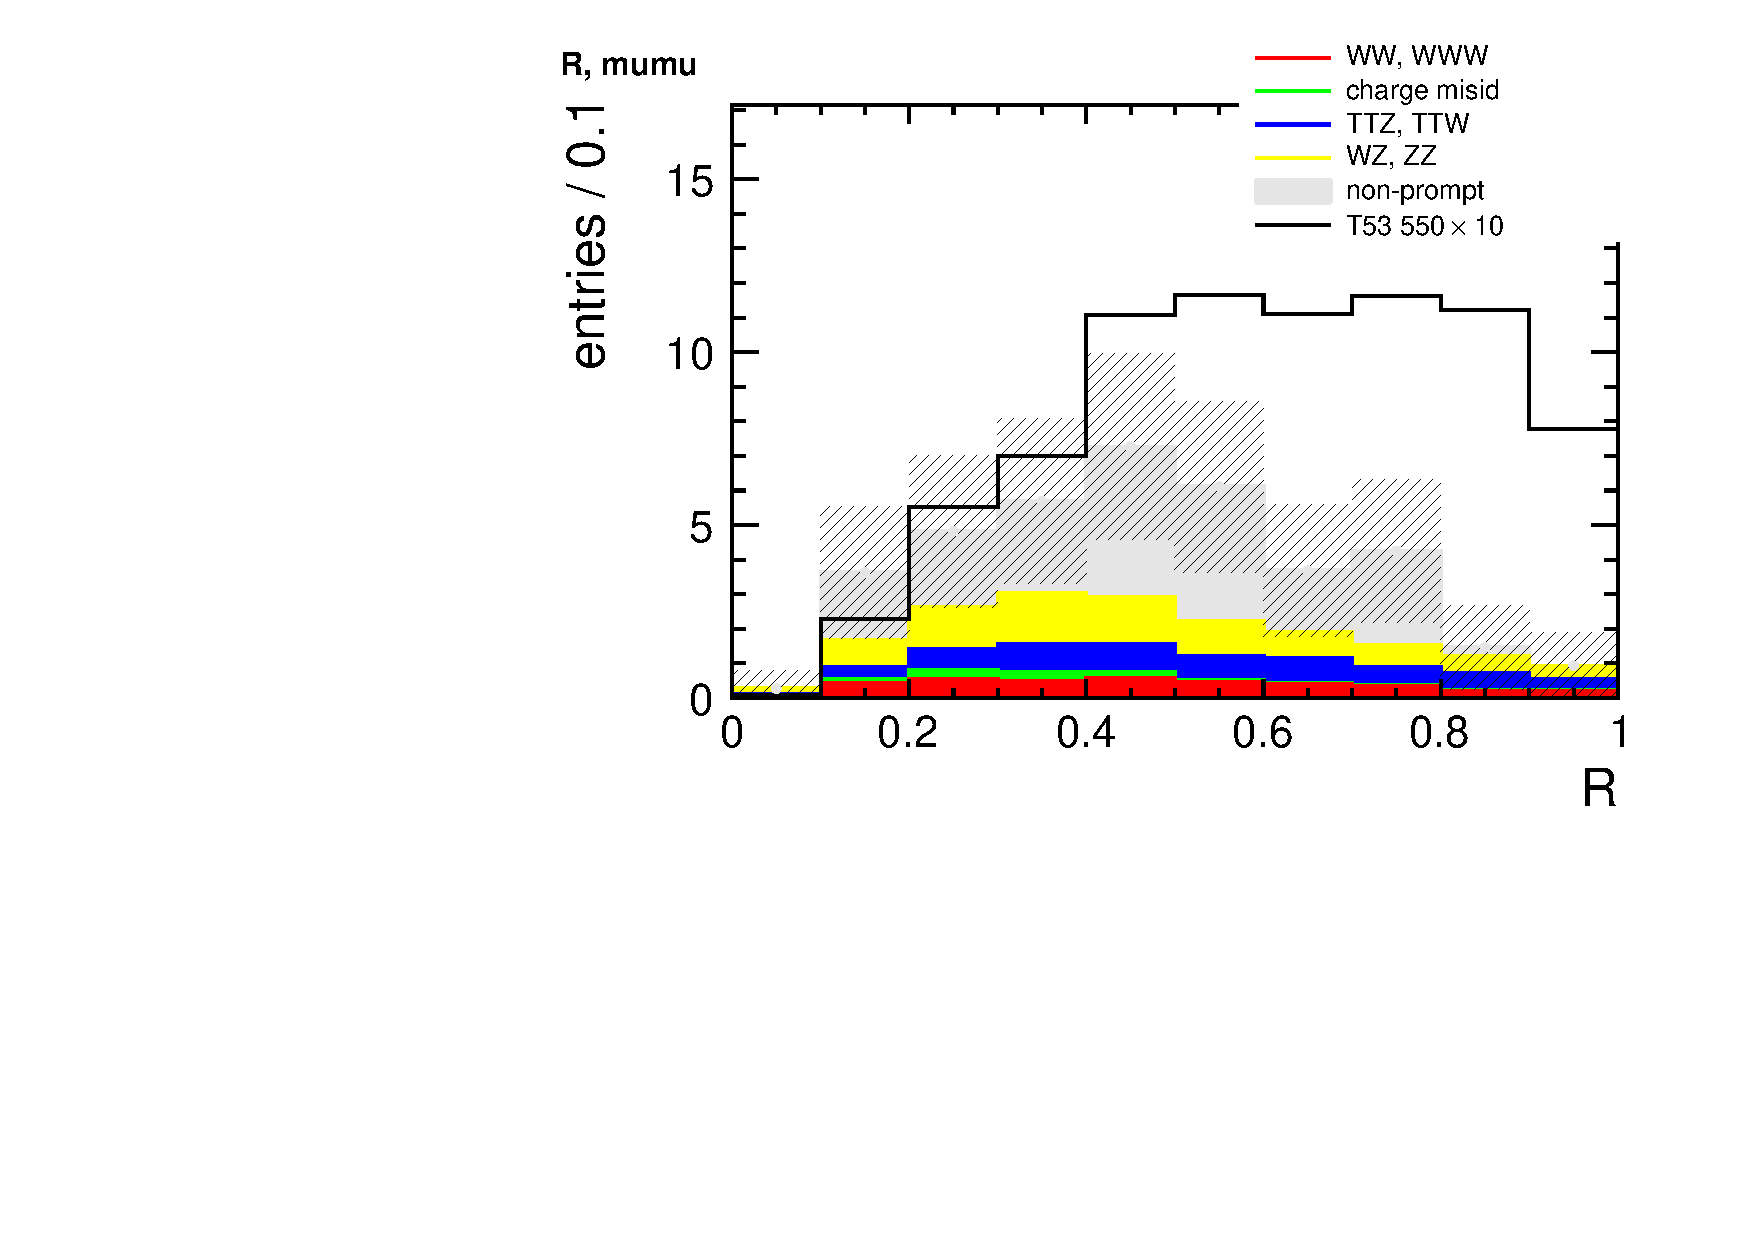
\includegraphics[width=.7\textwidth]{images/pdf/r_mumu_0}
    \caption{$R$ distributions for the three decay channels. Events with two same-sign leptons and at least
two jets are shown.}
    \label{fig:r_nobtag_app}
\end{figure}

\begin{figure}[htb]
    \centering
    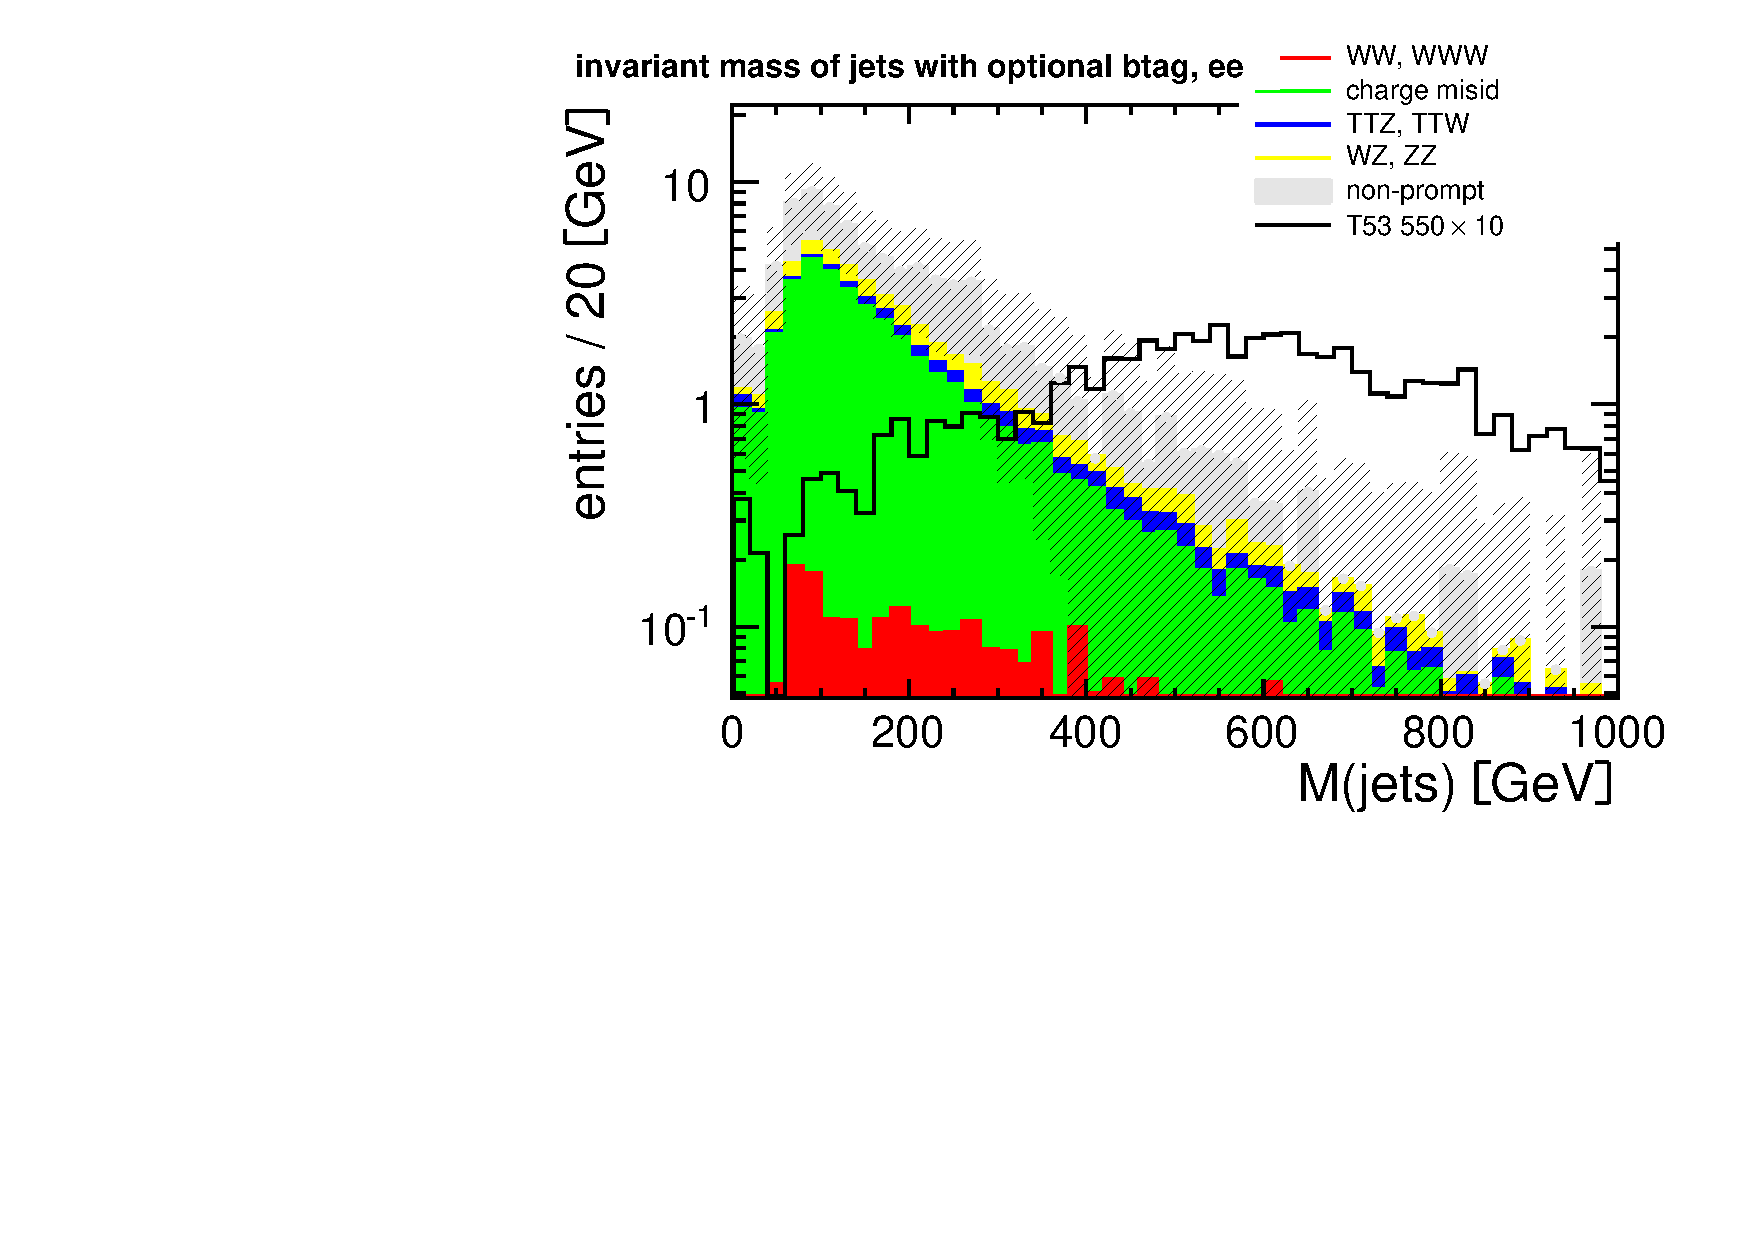
\includegraphics[width=.7\textwidth]{images/pdf/had_mass_optional_btag_ee_0}
    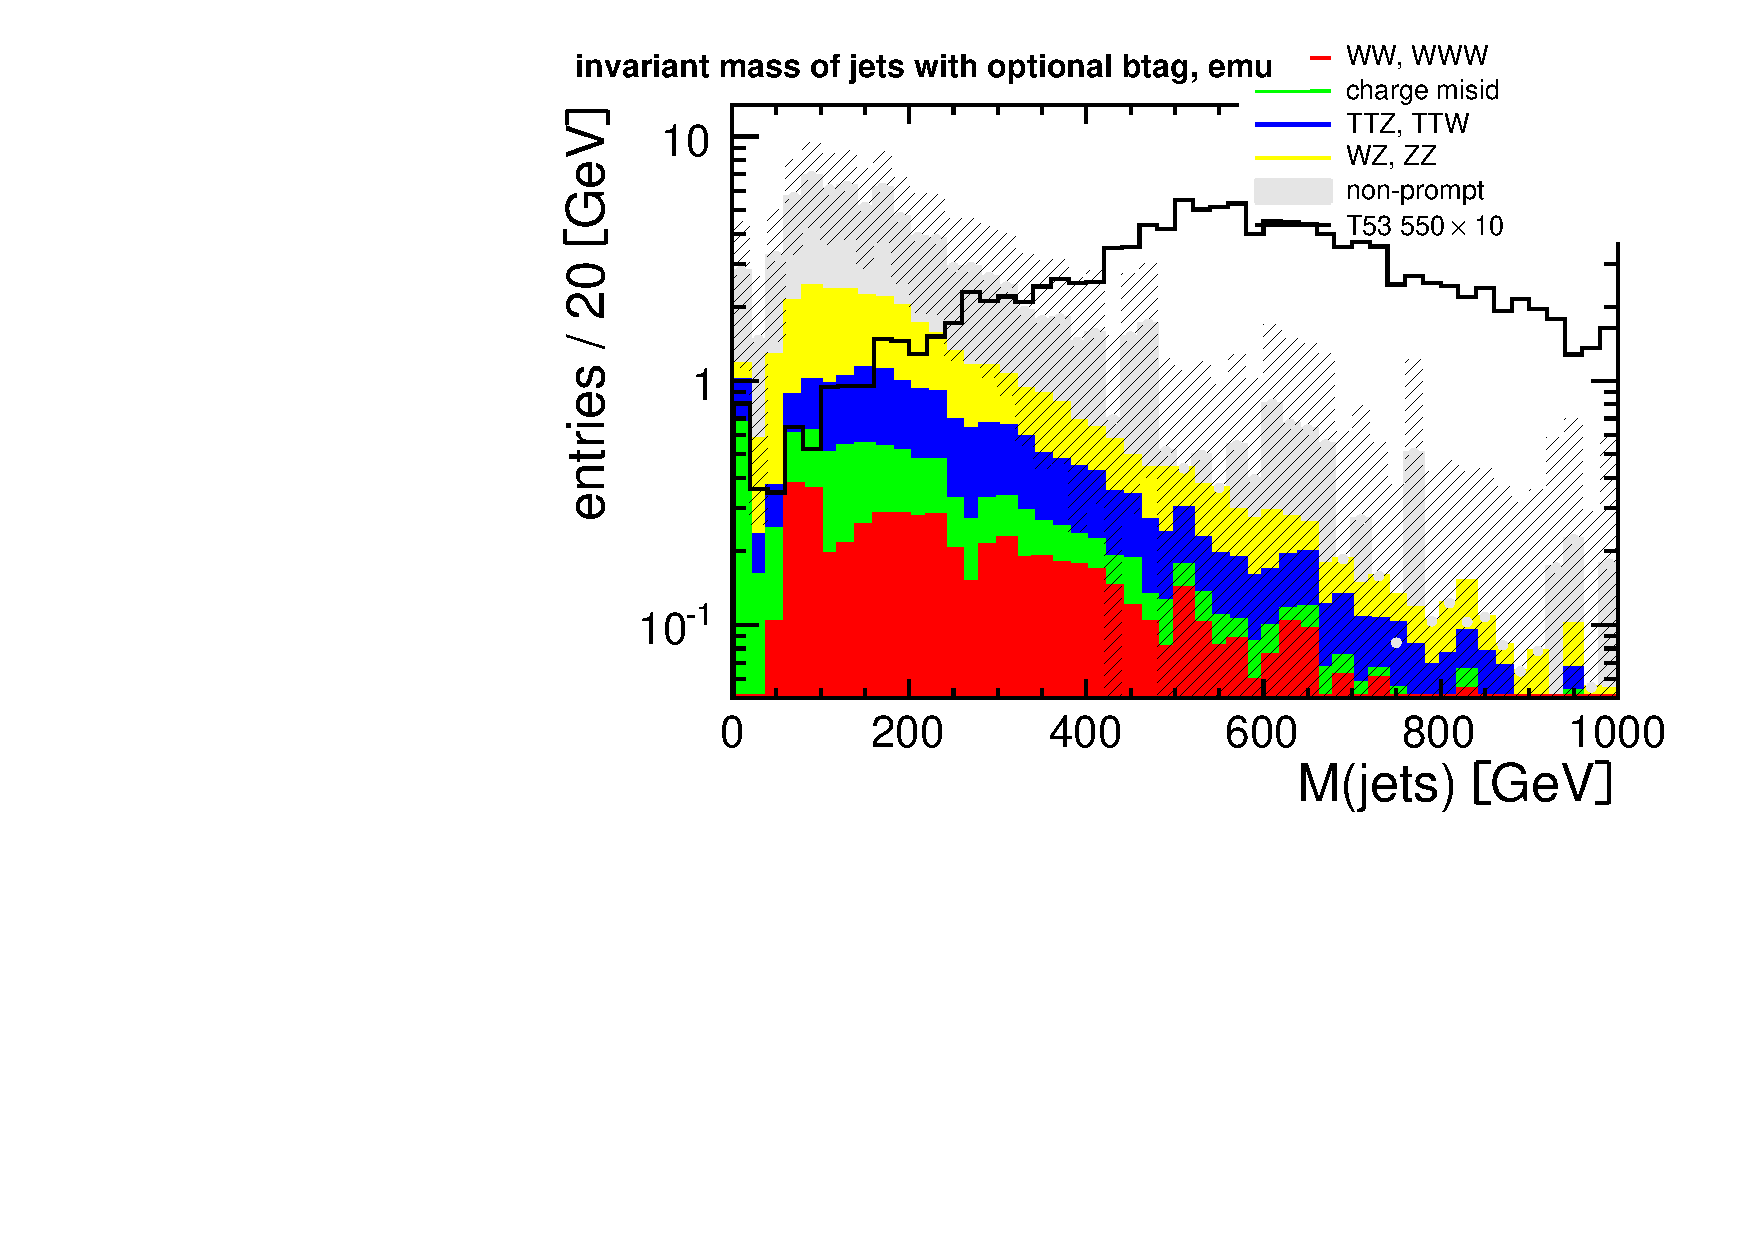
\includegraphics[width=.7\textwidth]{images/pdf/had_mass_optional_btag_emu_0}
    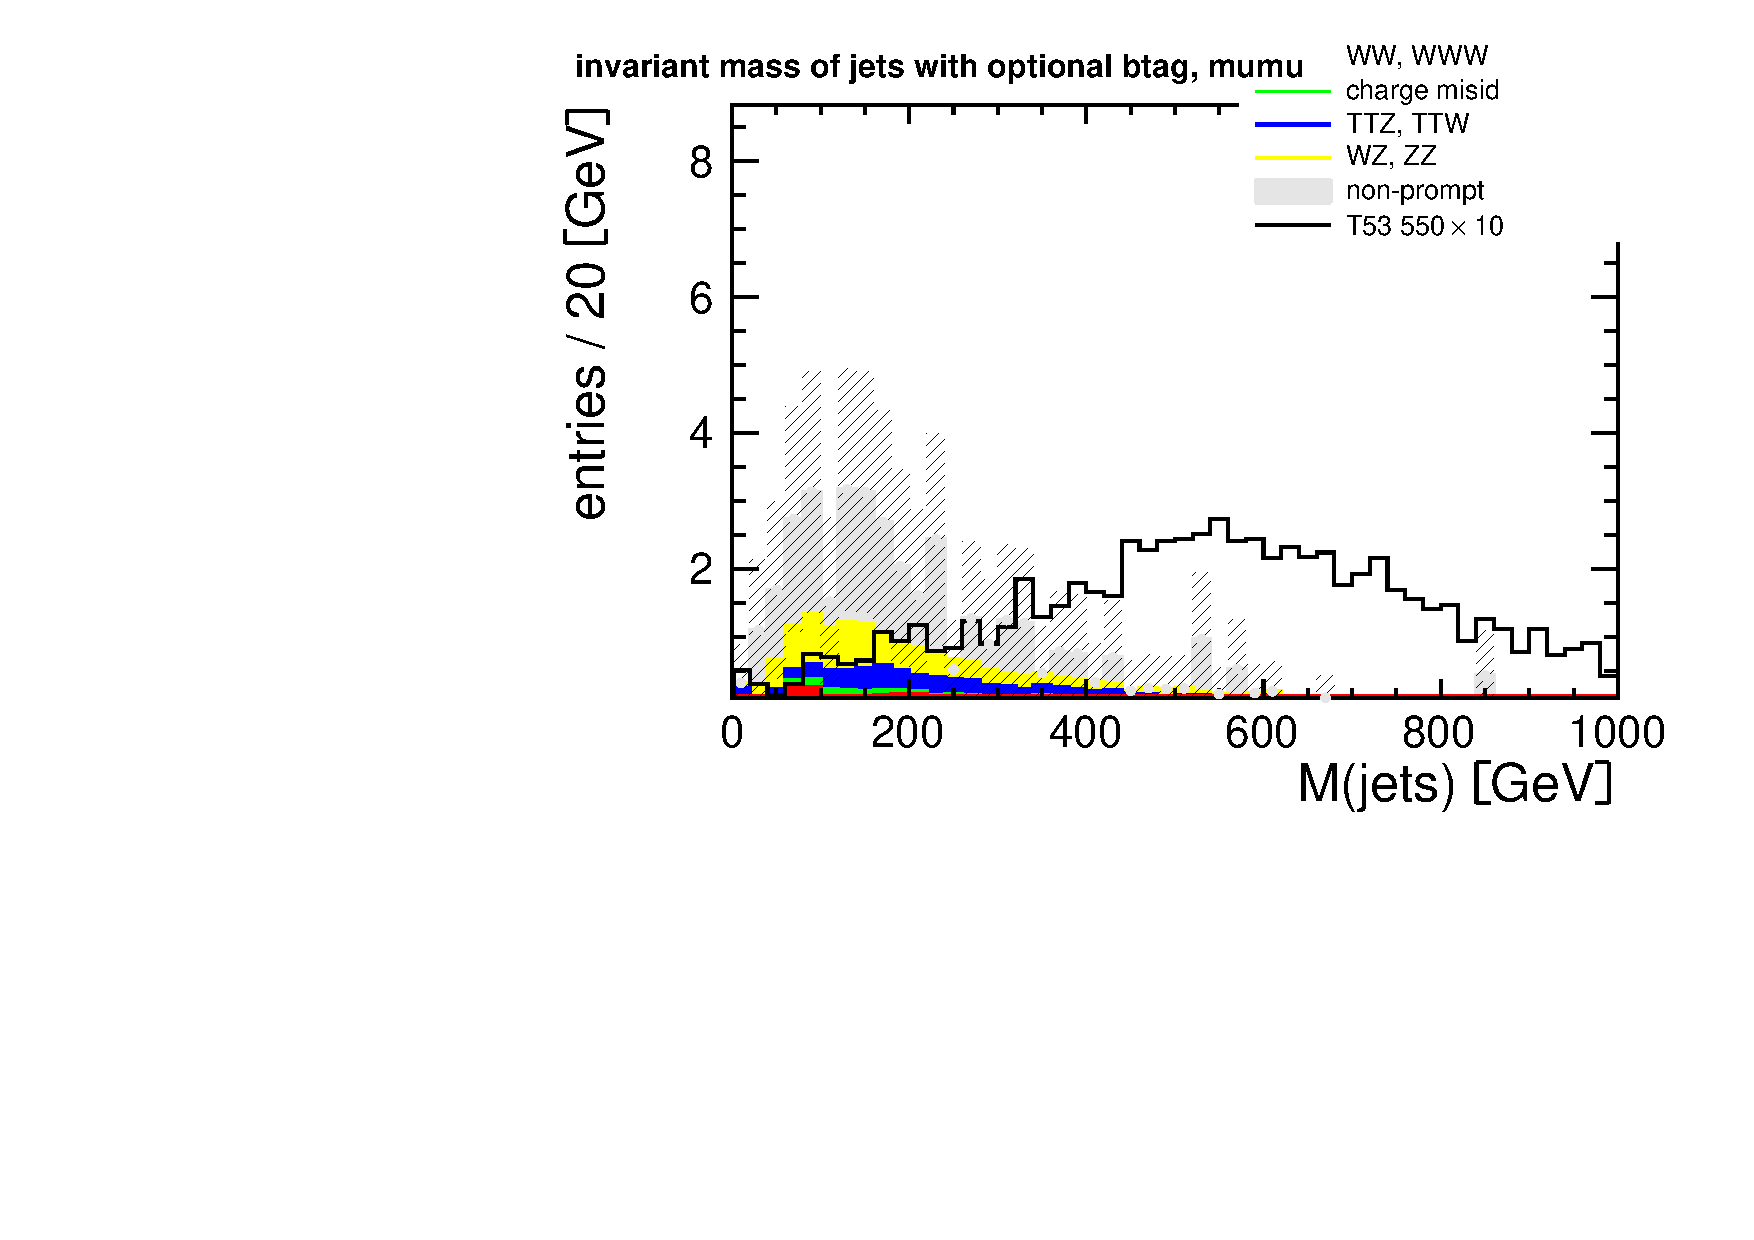
\includegraphics[width=.7\textwidth]{images/pdf/had_mass_optional_btag_mumu_0}
    \caption{Invariant mass of the hadronic system for the three decay
    channels, with the b-tag correction. Events with two same-sign leptons and at least
two jets are shown.}
    \label{fig:had_mass_optional_btag_app}
\end{figure}

\begin{figure}[htb]
    \centering
    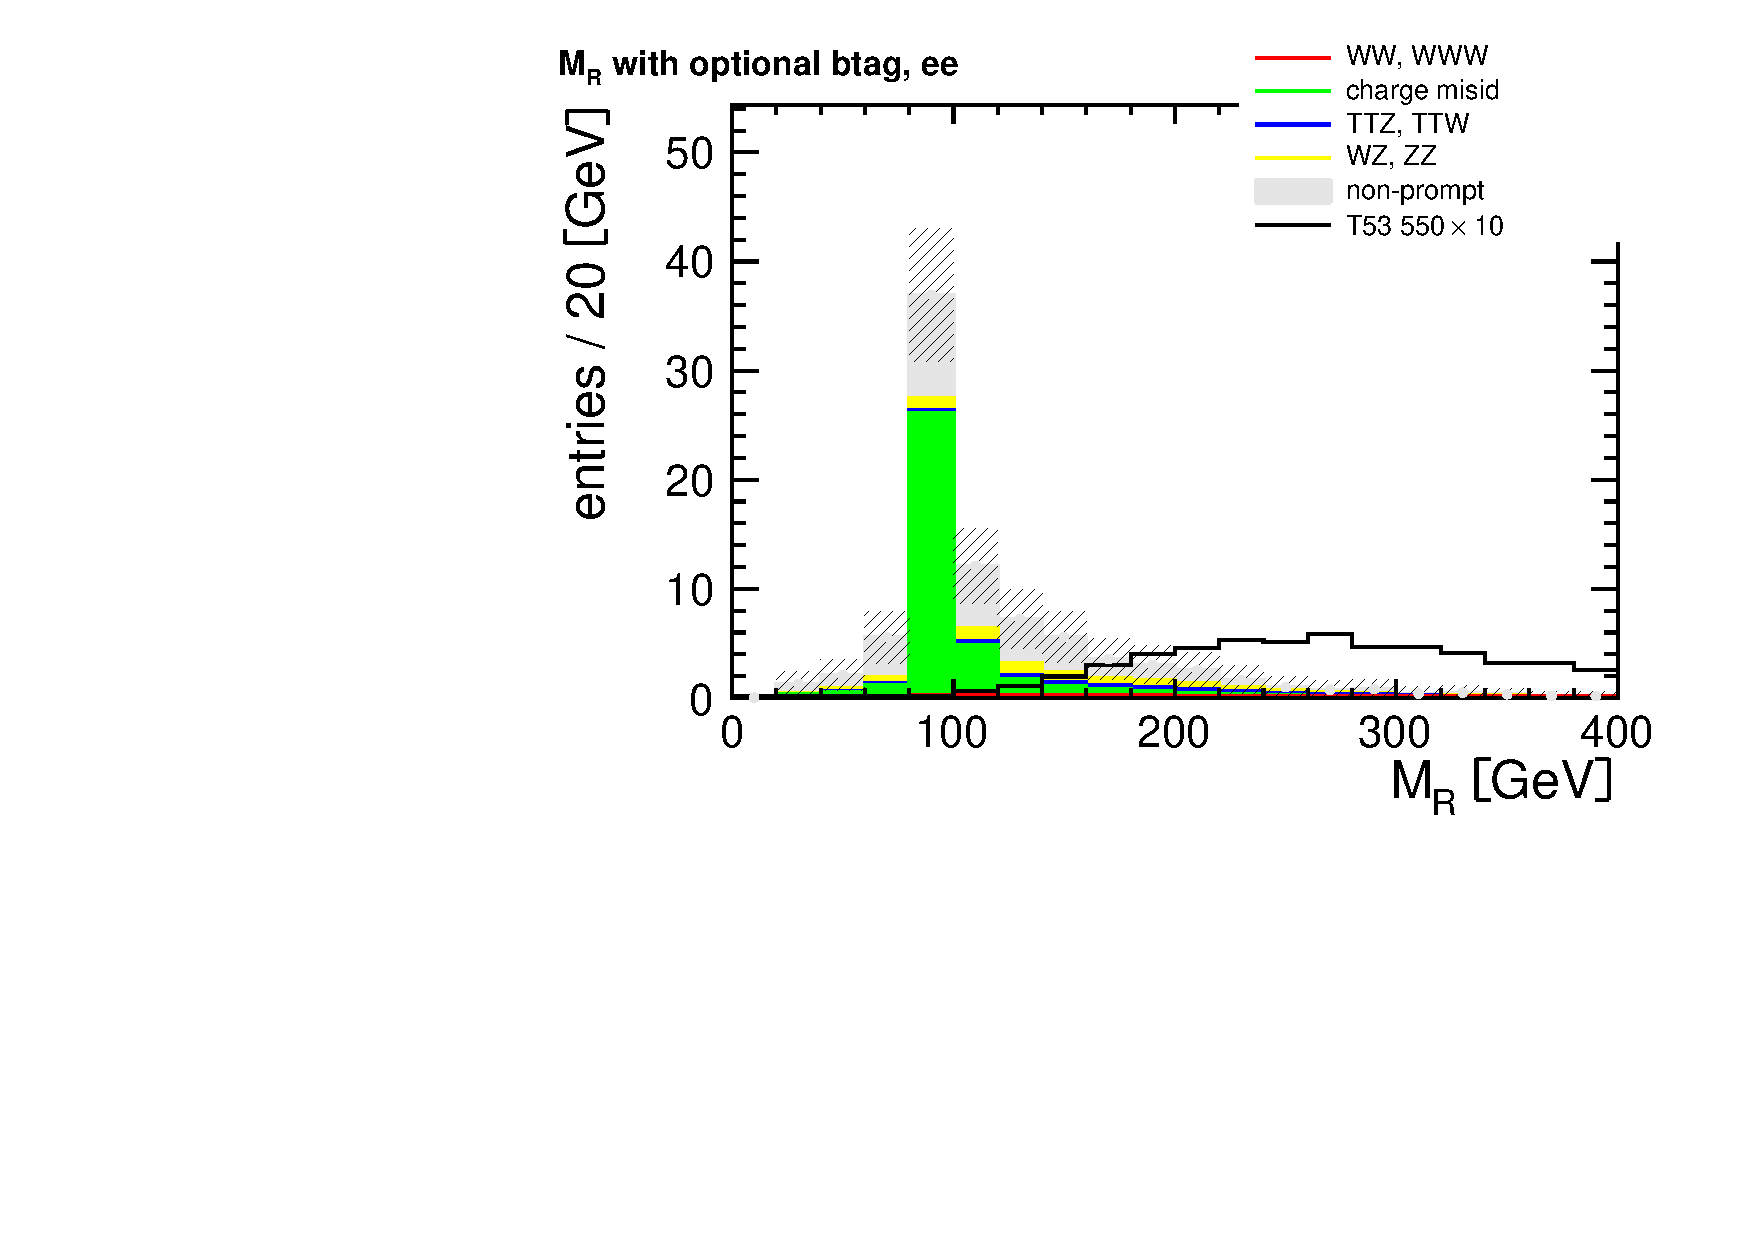
\includegraphics[width=.7\textwidth]{images/pdf/mr_optional_btag_ee_0}
    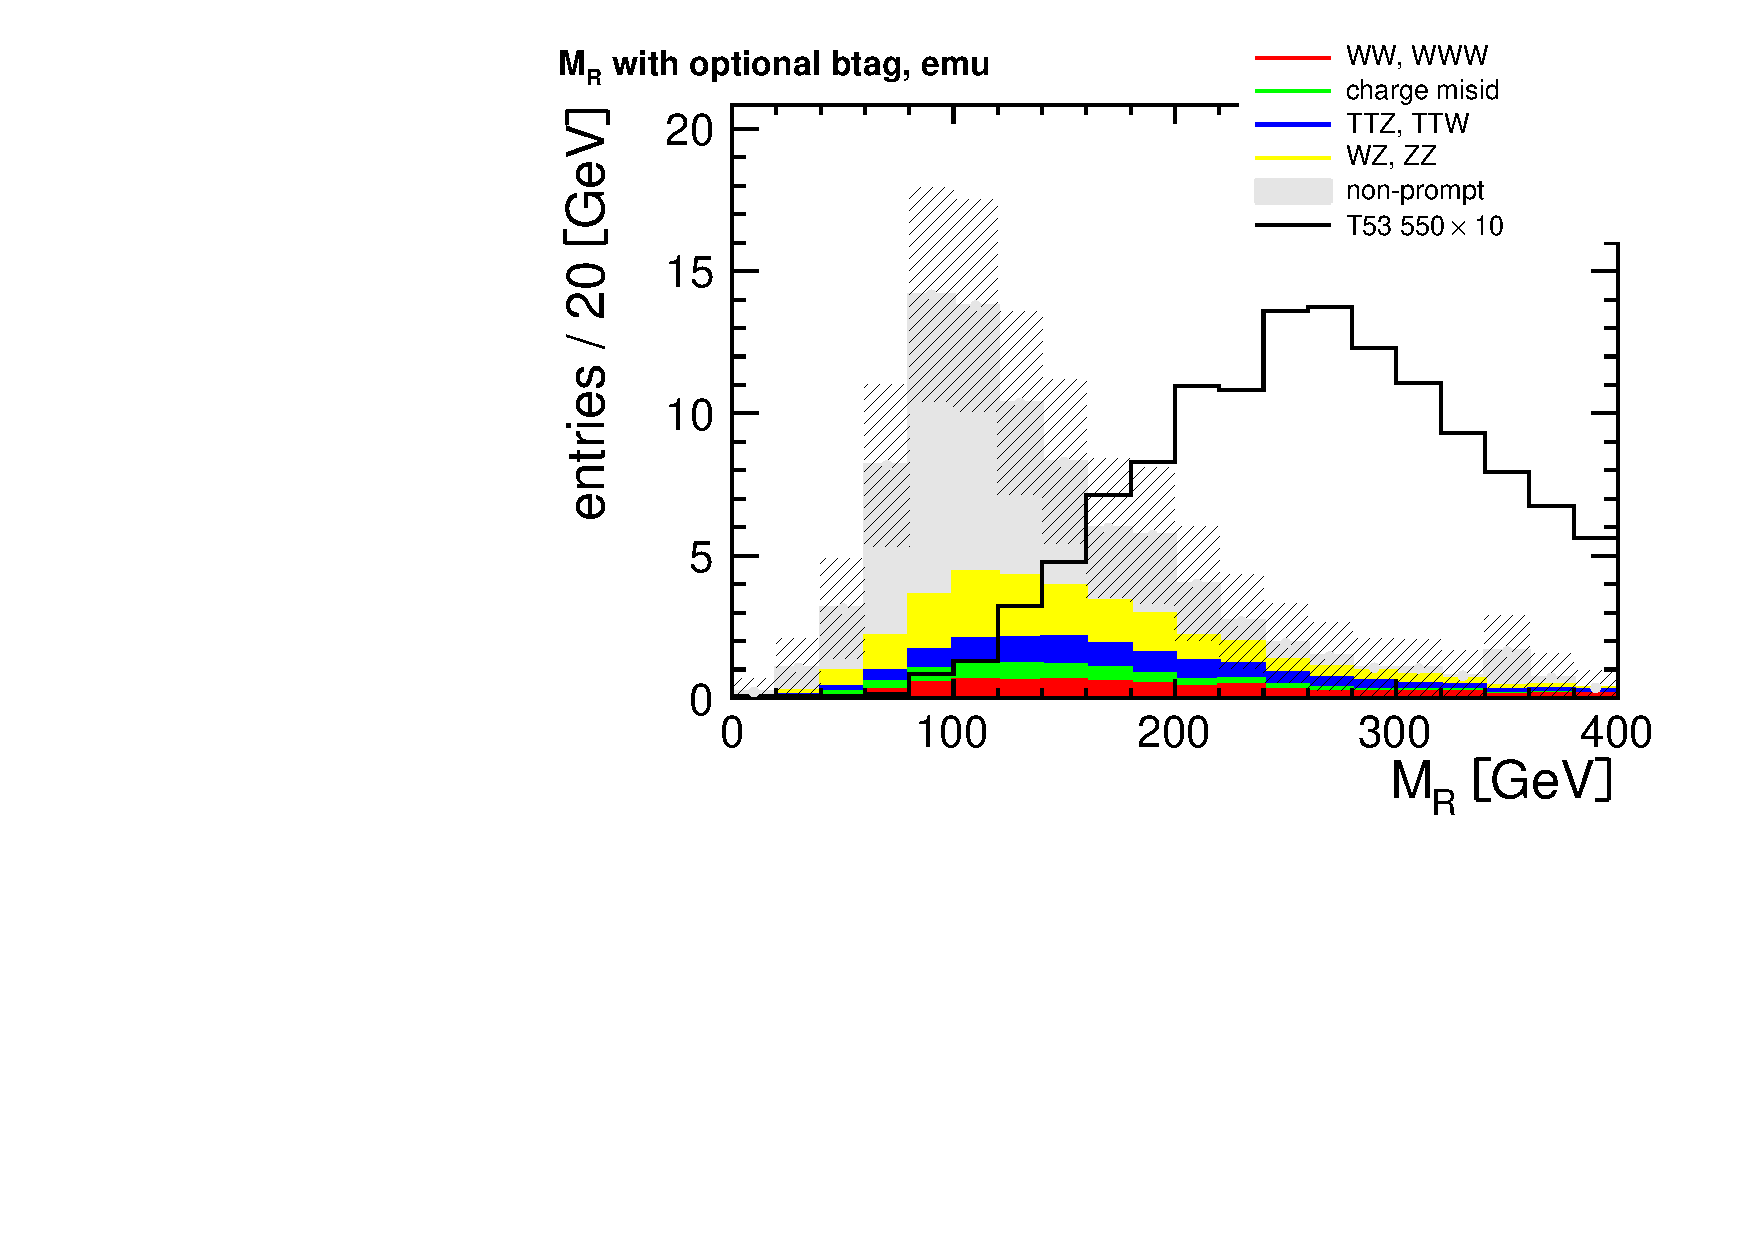
\includegraphics[width=.7\textwidth]{images/pdf/mr_optional_btag_emu_0}
    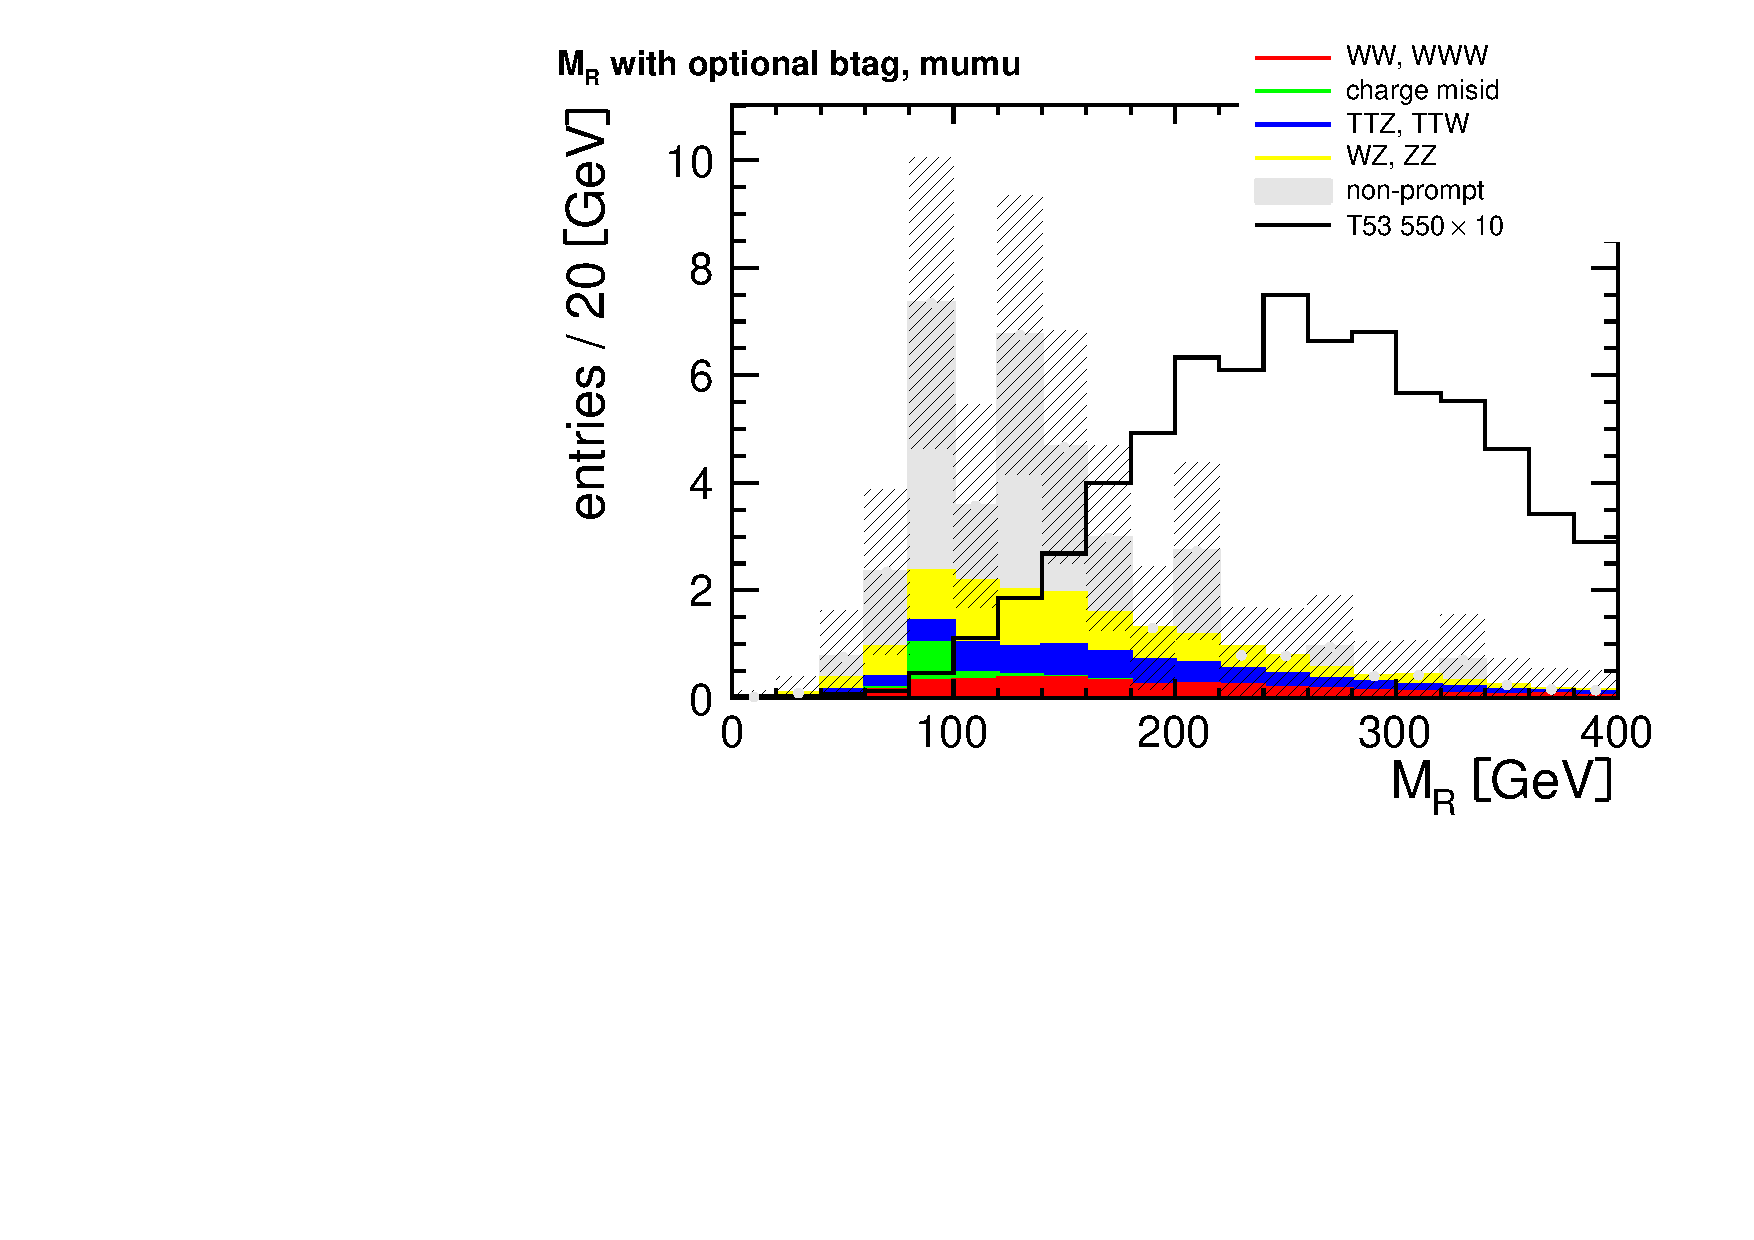
\includegraphics[width=.7\textwidth]{images/pdf/mr_optional_btag_mumu_0}
    \caption{$M_R$ distributions for the three decay channels,
        with the b-tag correction. Events with two same-sign leptons and at least
two jets are shown.}
    \label{fig:mr_optional_btag_app}
\end{figure}

\begin{figure}[htb]
    \centering
    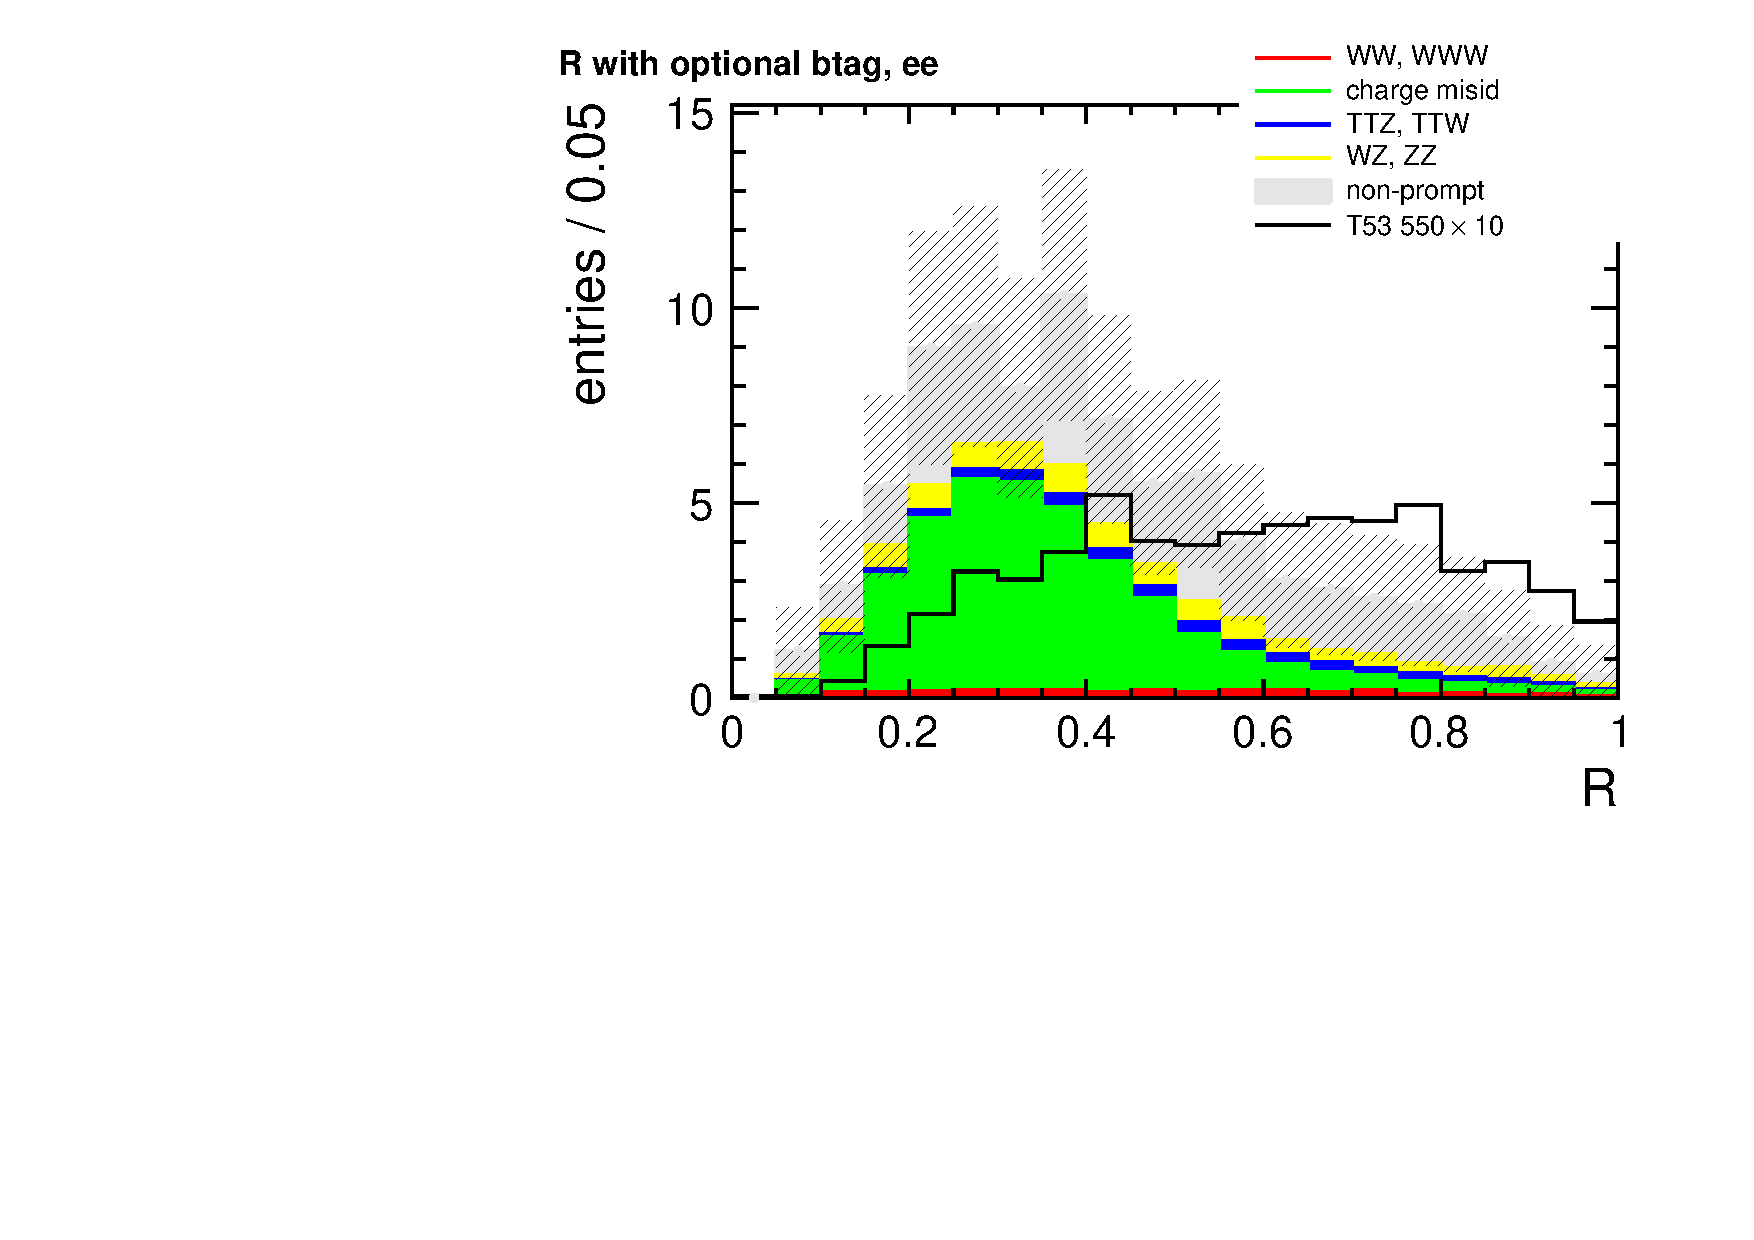
\includegraphics[width=.7\textwidth]{images/pdf/r_optional_btag_ee_0}
    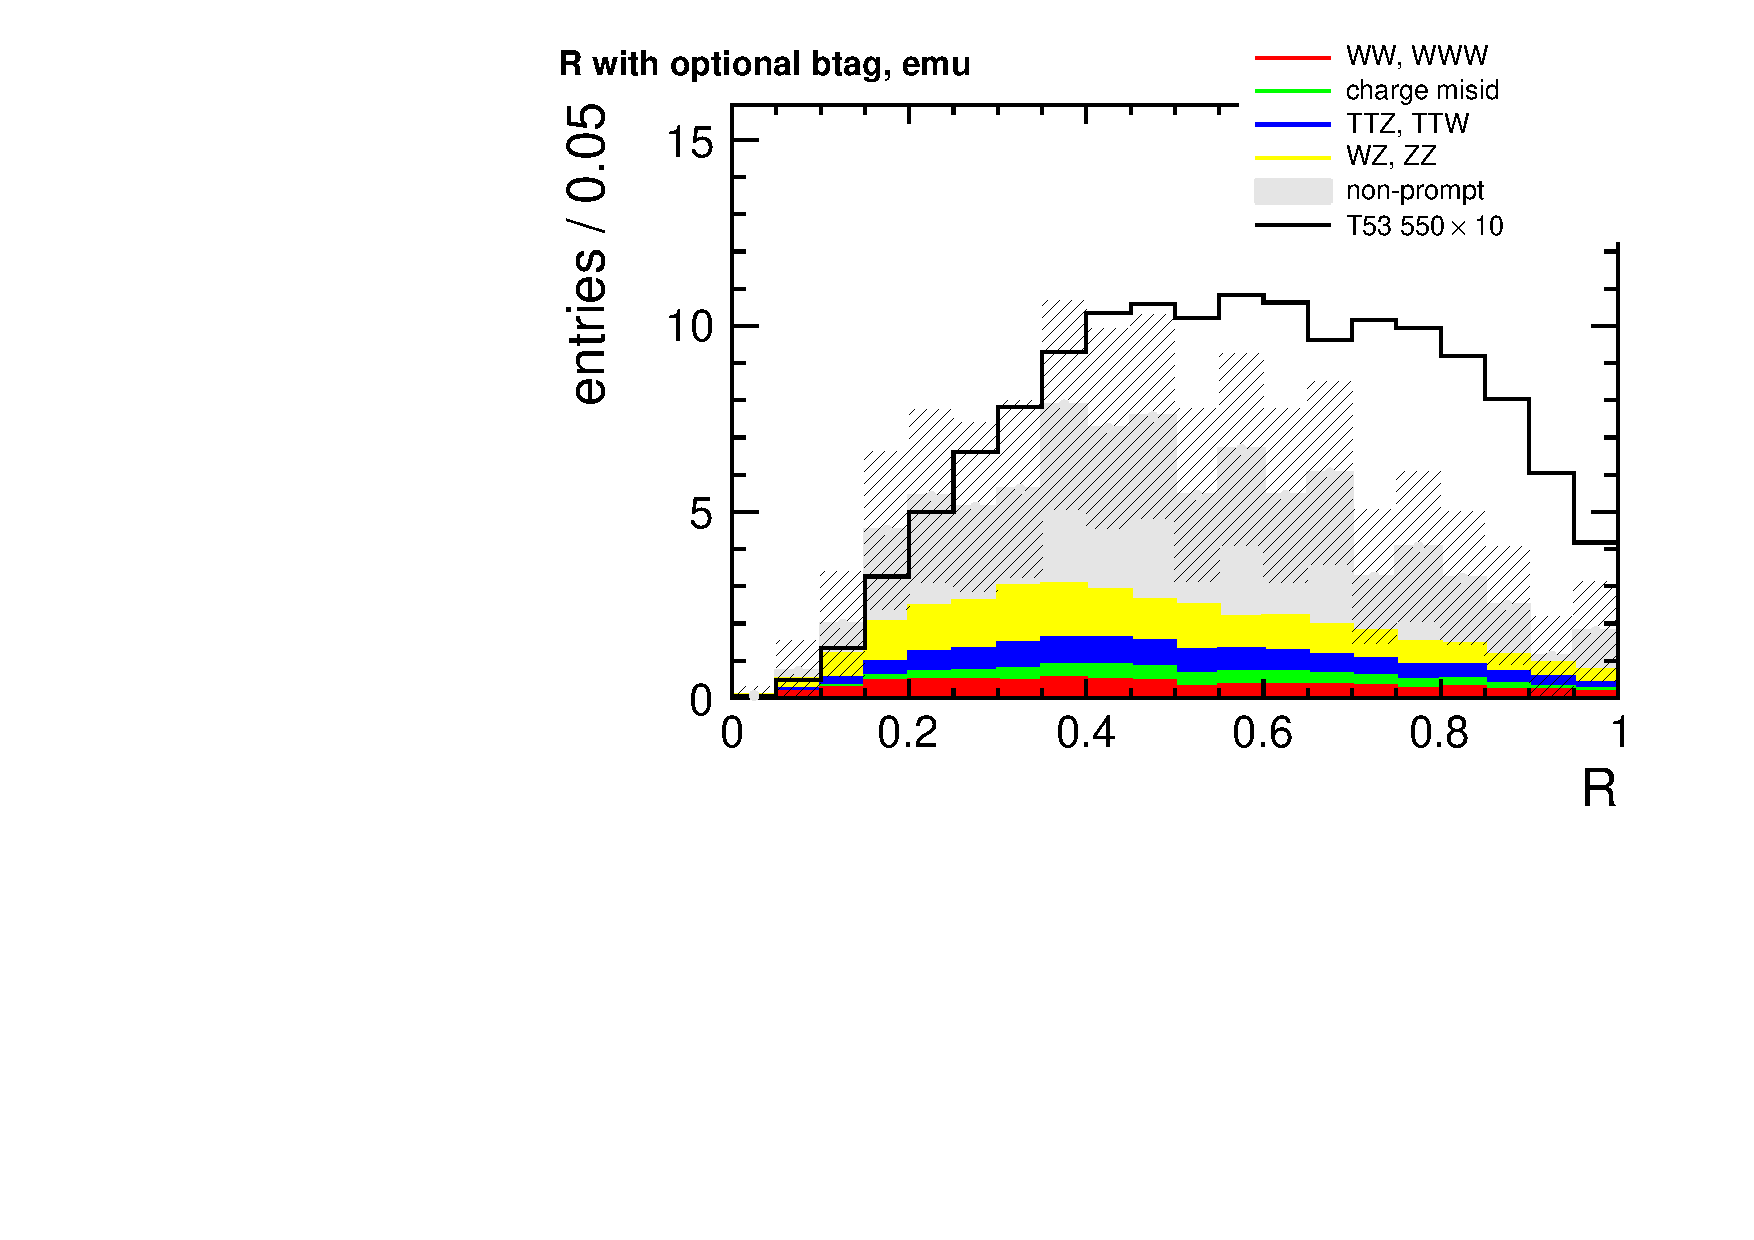
\includegraphics[width=.7\textwidth]{images/pdf/r_optional_btag_emu_0}
    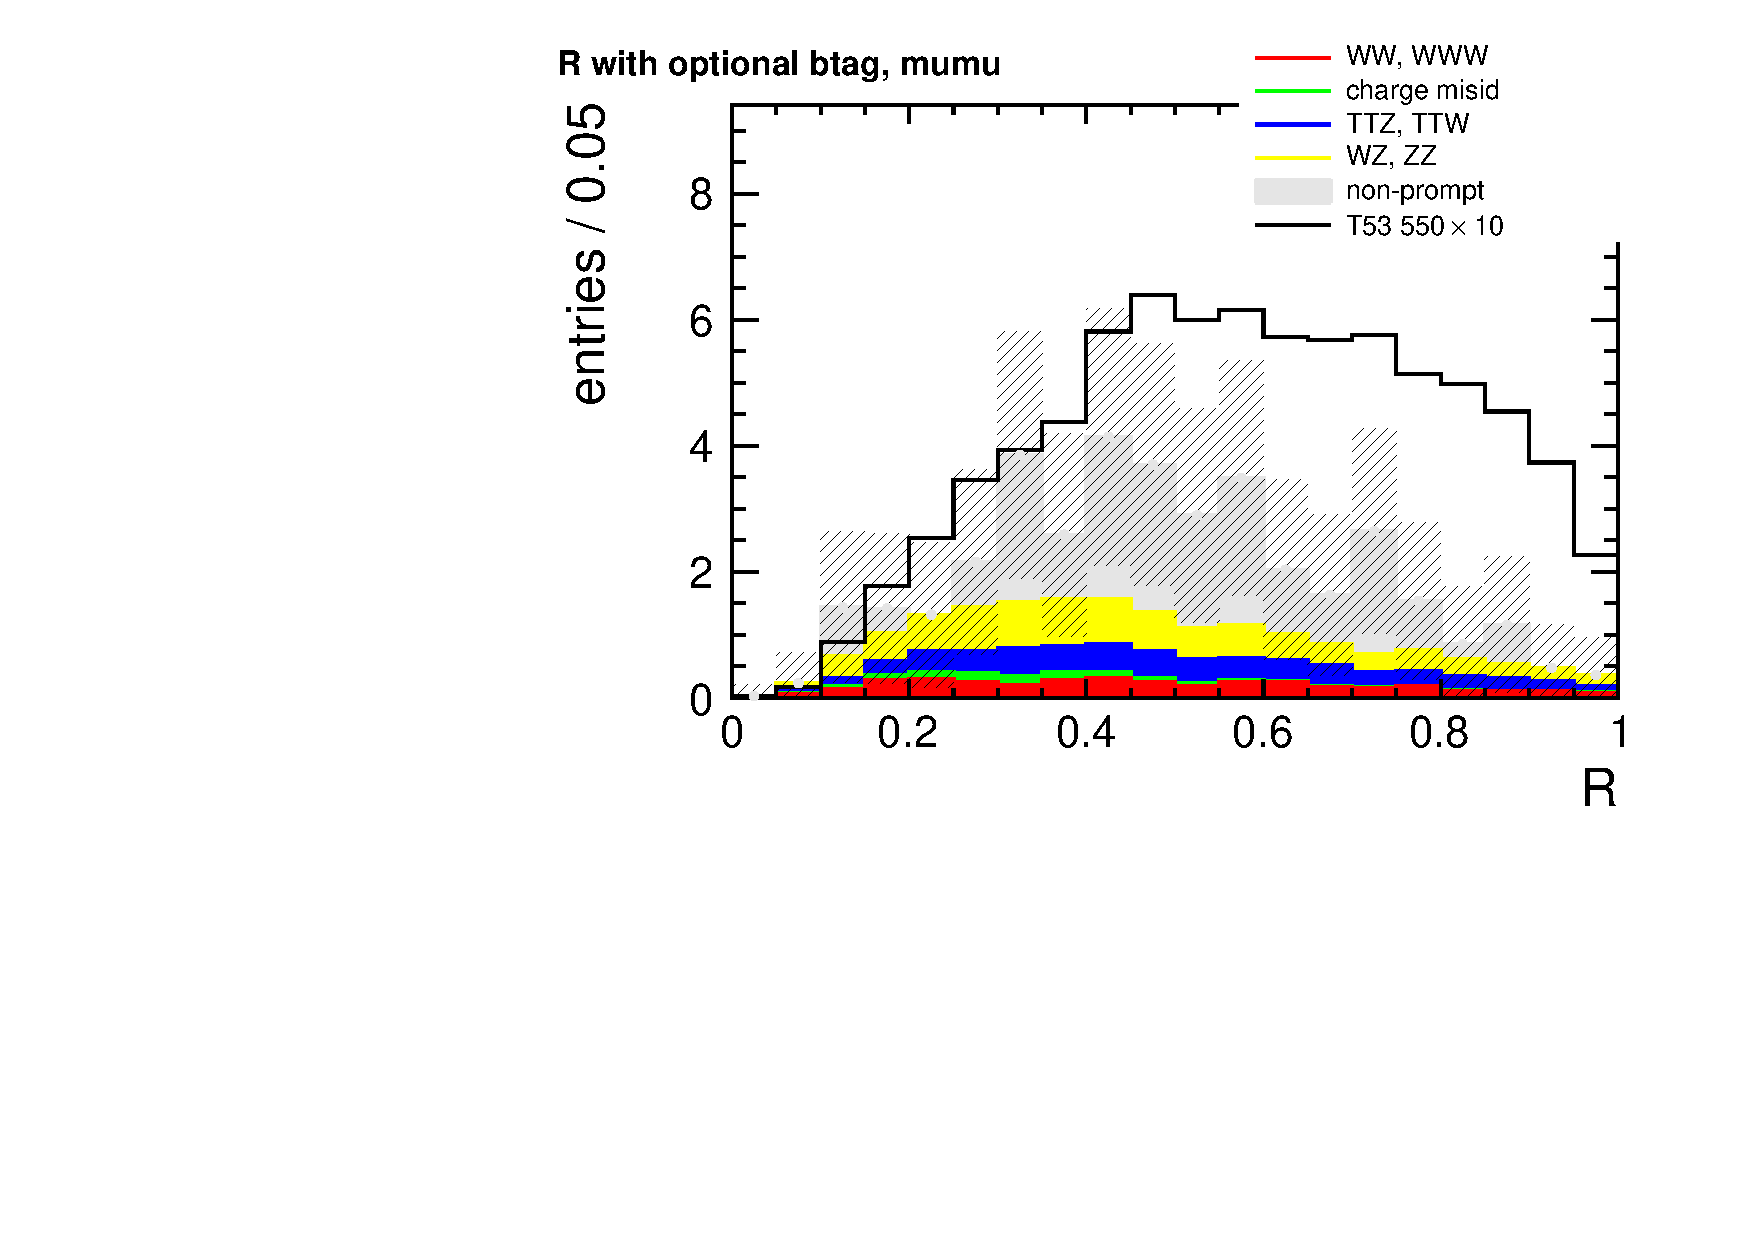
\includegraphics[width=.7\textwidth]{images/pdf/r_optional_btag_mumu_0}
    \caption{$R$ distributions for the three decay channels,
        with the b-tag correction. Events with two same-sign leptons and at least
two jets are shown.}
    \label{fig:r_optional_btag_app}
\end{figure}

